\documentclass{article}
\usepackage{graphicx}
\graphicspath{ {images/} }
\usepackage[english]{babel}
\addtolength{\oddsidemargin}{-.875in}
\addtolength{\evensidemargin}{-.875in}
\addtolength{\textwidth}{1.75in}
\addtolength{\textheight}{1in}
\usepackage[utf8]{inputenc}

\begin{document}
\begin{titlepage}
    \centering
	{\scshape\LARGE Written Report Design 2016 \par}
	\vspace{1cm}
	{\scshape By: Cheyenne Fye, Brett Hladczuk, Marcin Wisniowski \par}
	\vfill
	{\scshape December 10, 2016\\Stevens E-121\\Section Q Group 1 \par}
	\vspace{.5cm}
	{\scshape supervised by \\Dr. Joseph Miles \par}
    \vfill
% Bottom of the page
	{\scshape “I pledge my honor that I have abided by the Stevens Honor System.”\par}
\end{titlepage}

\pagenumbering{roman}
\section{Abstract}
The objective of this project was to build a fully-functioning robot to follow light sensors and demonstrate its efficiency against our fellow classmates in a competitive scene. By following the guidelines of design, construction, and programming of the robot, the robot was effectively created to fulfill its role in the competition. Although there was some prior knowledge, most of the engineering techniques consisting of mechanical, electrical, software, and management engineering were learned as the process continued throughout the semester. Working on the project involved planning ahead, combining ideas, communicating, and attacking each challenging obstacle as a group. In the end, Group 1 earned a total of  points that resulted in place out of eight groups.
\newpage

\tableofcontents
\newpage

\pagenumbering{arabic}
\section{Introduction}
\subsection{Purpose}
	The purpose of this report is to explain the methods the group utilized in order to derive the final design for the robot, as well as allows Group 1’s design to be effectively compared to other groups. This report provides a single document to explain the decisions made within the group in choosing programming methods, design specifications, and material choices. Finally, this report documents the way the group adapted to problems encountered and can be used by the professor to make future projects easier for students.
\subsection{Background and Objectives}
\begin{itemize}
  \item Introduce you to a Project Design and Development environment where you will experience typical design problems and employ problem solving techniques
  \item Instill the importance of a program plan and program management skills
\item Enable you to experience the group dynamics associated in a team project where everyone has their own tasks to integrate into the whole project
\item Provide an application for the design and construction of a Solid Works designed component (Robot LOGO) that can be milled on the computer numerically controlled (CNC) machine
\item Create a friendly competitive atmosphere to foster innovation and success oriented thinking
\item Introduction to a wide of variety engineering areas, i.e. software design and development using: 
    \begin{itemize}
        \item C language
        \item Mechanical Design
        \item Electrical Design
        \item Software/Hardware Integration Techniques
        \item Strategy Development
        \item Hands on Construction Skills
        \item Use of Industry Standard Software Applications (Project, Word, PowerPoint, Visio, Solid Works) 
    \end{itemize}
\end{itemize}
\subsection{Project Specifications}
\begin{itemize}
    \item Develop a “Win Strategy”
\begin{itemize}
    \item Understanding the competition objectives and the available suite of sensors, and anticipating all the things that can happen or go wrong, you must define your robot strategy. Think through a typical competition. How do you start? What do you do first, second? What if you bump into something? How do you know what you bumped into? How do you know where you are? How do you know where your opponent is? Do you care? What will make your robot unique and give you a competitive edge? All of this “strategizing” should result in a definition of the sensor suite and a top-level program flow that can be used to schedule tasks based on a better understanding of the complexity and level of effort required.
\end{itemize}
\end{itemize}
\begin{itemize}
    \item Design/Construct/Test the “Floor Sensor Module”
\begin{itemize}
    \item Construct mechanical housing to hold FSM LED and photo sensor components b. Design/locate/interface FSM LED circuitry and specify the I/O pin that will be used to interface to the microcontroller
\end{itemize}
\end{itemize}
\begin{itemize}
\item Mechanical Design
\begin{itemize}
\item Decide whether your robot will use front wheel drive, or rear wheel drive.
\item Decide where/how to mount the electrical bumper switches.
\item Design the physical bumpers and how they will connect to the bumper switches
\item Design and integrate the “Floor Sensor” module into robot chassis design
\item Design physical mounting of all light sensors and any optional sensors you may have chosen to include
\item Design LOGO plaque and mounting
\end{itemize}
\end{itemize}
\begin{itemize}
    \item Electrical Design
\begin{itemize}
    \item Design/layout printed circuit boards to hold FSM LED and associated electrical components.
\item Design/layout printed circuit boards to hold and connect bumper switches.
\item Design/document microcontroller interface design and wiring diagrams for additional sensors (i.e., which spare I/O pins will control which sensors, which pins will they physically connect to on the microcontroller board?)
\item Design wiring routes and tie back points to ensure safe/sturdy connections
\end{itemize}
\end{itemize}
\begin{itemize}
    \item Software Design and Integration
\begin{itemize}
    \item Develop a Software Integration Plan (SIP) that sequentially builds up the robots capabilities (i.e., write a program to make the robot move straight and test it, then add the capability to avoid obstacles by sensing bumper contact closures and test it, then develop the movement algorithm the robot will use to seek light and test it, etc).
    \item Demonstrating incremental capability via an organized testing strategy is an extremely important concept in complex software/electronic hardware designs.
    \item Develop a flow chart for all software logic, following the SIP. The flow chart will be a living document that gets updated and refined when new features are added, or testing results in design changes. Two flowcharts will be necessary, one for the Main loop function and one for the Interrupt function.
    \item Code (in C) and test functional segments of code as they are completed. Testing code that interfaces with hardware in known as “Hardware/Software Integration”. A very structured, hierarchical test plan is essential to successfully get your robot working. A top level test plan will be provided to you.

\end{itemize}
\end{itemize}
\begin{itemize}
    \item Design LOGO using Solid Works and Construct using Plexiglas milled on the CNC (Computer Numerically Controlled) machines.
\end{itemize}
\begin{itemize}
    \item Final Prototype Testing/Debug via test runs in the arena
\end{itemize}

\subsection{Robot Mission}
The robot was designed to perform code in a rigid arena. However, because there could be variety in its placement for the starting position, the code had to stay dynamic and interactive with the environment. The robot's objective was to locate, approach and "knock out" two separate lights on the opposite side of the field from where it was placed. The robot to knock out the two enemy targets first, without knocking out their own, will be the winner of that competition. 
\subsection{Arena}
The competition will be held in a 4 ft by 8 ft “arena”. The arena will have 4-inch walls around the perimeter.  One half of the arena surface will be painted flat black, the other half reflective white to simulate home and enemy territories.  Your robot will be placed into the arena on your home territory, but you will not know in advance the color of your home territory. \\

The arena is supported by two “types” of lights, one directional light used for navigation and four target lights, two enemy and two friendly.  The navigation light is located 30” above the direct center of the arena.  A light sensor on the robot pointed upwards can seek this light to get direction. The target lights will be located at arena floor level somewhere along the perimeter of the arena. Their positions can vary and will not be known in advance. Target lights on the arena have switches associated with them, such that prior to running into a target light, the robot will run into the switch.  The arena micro controller will detect the switch closure, turn off the associated light and turn on a second light in a different location. \\

Obstacles (3” high wooden shapes) will be located within the arena. The robot must use its collision avoidance subsystem (bumpers) to detect when these obstacles (as well as the arena perimeter walls) are hit to make course corrections. The location of obstacles will be known in advance. Two robots compete simultaneously in the arena. 

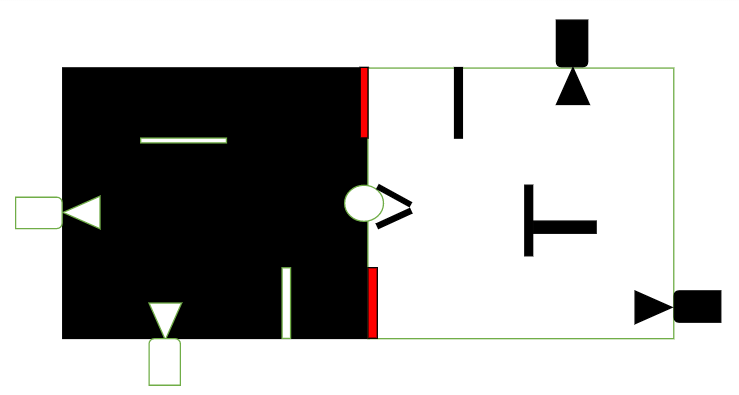
\includegraphics[width=\textwidth]{Arena.png}
\subsection{Project Planning}
Group 1 created a Gantt Chart to help organize the project and plan ahead each of the sections and subsections. The project was split up into separate sections of Hardware, Software, Testing and Integration, and Project Planning. Since it was our first time working with this type of project our time for each of the objectives was doubled to account for learning and errors that would occur.\\
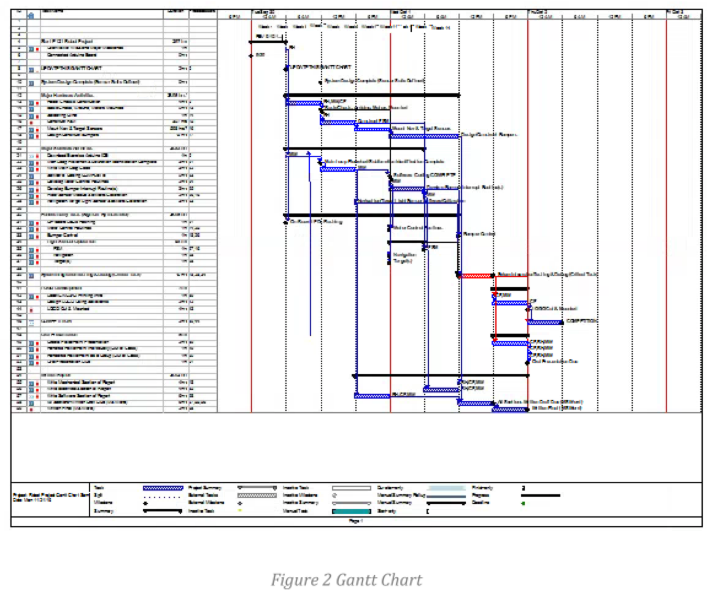
\includegraphics[width=\textwidth]{Gantt_Chart.png}
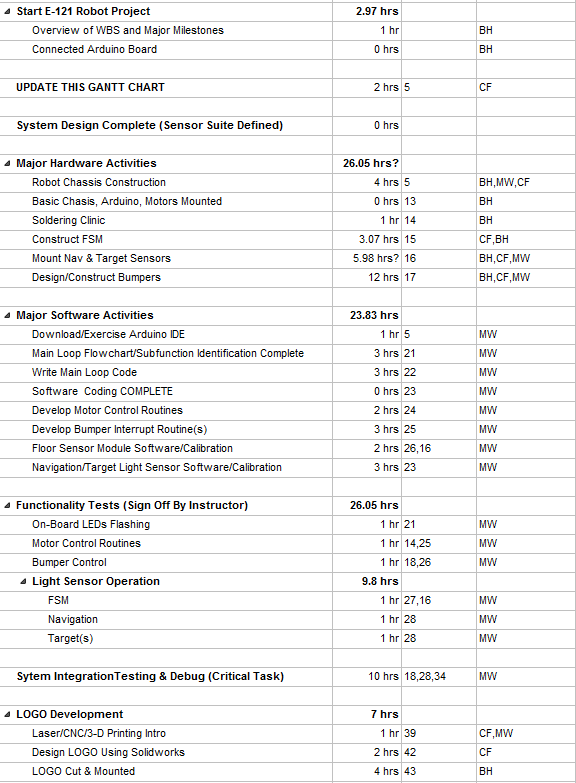
\includegraphics[width=\textwidth]{GanttChartBreakdown.png}
\subsection{Roles}
Group 1 split its members into different sections of work to maximize efficiency. The members were split between Hardware, Software, and Electrical Design and Implementation, as well as a Project Manager.
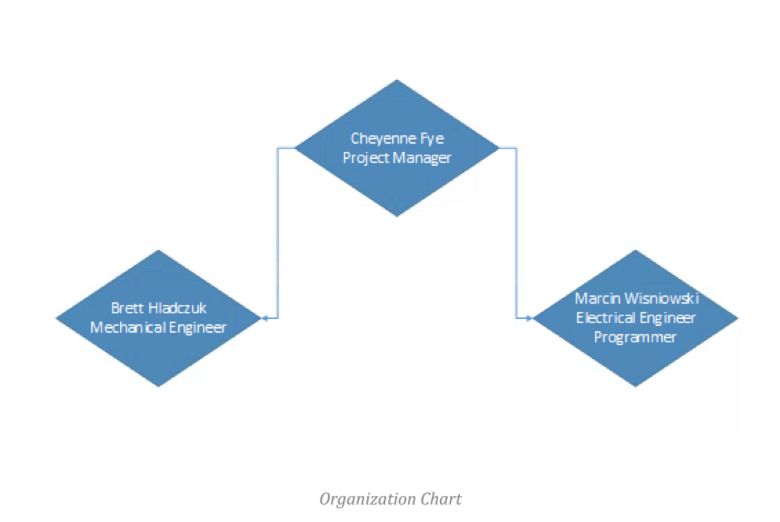
\includegraphics[width=\textwidth]{Organization_Chart.png}

\newpage
\section{Discussion}
\subsection{Requirements}
    The objective of the robot to navigate around an arena and eliminate two enemy targets in the shortest amount of time. \\
    
    The robot started a different colored territory than its opponent, with a rule stating that the color of home court would not be known in advanced. In order to make sure the robot knew what side of the arena it was on, the team created and installed a floor sensor module. The group decided that the robot should have it's body entirely across the territory boundary to consider it in enemy territory. This was considered the safest strategy as rotating on the boundary would not affect the robot as drastically. \\

    The team also decided to incorporate three light sensors to allow for more data collection and analysis in order to strengthen our decisions made in the code. The light sensors allowed the robot to detect the lowest value (brightest light) and fixate perfectly on it by comparing its value with the other light sensors. Another rule of the competition was that the location of the two target lights that the robot had to switch off were unknown in advanced. Because of this, a lot of movement needed to be decided dynamically with the information collected by the light sensors. \\

    Likewise, the robot had a beacon light connected to the back that was utilized whenever the robot was on its home side and was trying to find its way to the enemy’s territory. The beacon was placed at the back to strengthen the robots precision when closer to the beacon, so that until it was fully over the boundary it would have strong readings on the beacon and not be shielded. \\
    
	Finally, two bumpers were designed and attached to the front of the robot in order to turn the motors on and off when the robot ran into the walls of the arena. Since no modifications could be made to the chassis, the bumpers were mounted to the front of the robot and made to wrap around the front of the robot. The two bumpers were necessary for the robot to help it navigate around obstacles. When the left bumper was hit, the robot backed up to the left and when the right bumper hit, the robot backed up to the right. When both bumpers hit the walls of the arena, the robot moves backward, detects where the brightest light is located, and turns toward the brighter light. The group decided to incorporate going backwards with turning simultaneously in order to save time. The speed of the robot was kept constant throughout the program, however because no modifications could be made to the motors, our group did not focus too much on being taken advantage of this aspect.
\subsection{Rules and Regulations}
The following rules and information must be used to guide the design of your robot and your competitive strategy:
\begin{itemize}
    \item No modifications are allowed to the two 1/4 inch thick gray plastic mounting platforms that provide the frame for your robot. These frames will be reused next year and must not be altered in any way. The lower platform has the motors and gearbox attached to it. The upper platform has the microprocessor board attached to it. Sandwiched in between these two mounting platforms is the battery. You cannot glue or epoxy to these platforms. Along the entire perimeter edge of these two platforms, holes have been drilled roughly every half inch. Any of these holes may be used as connection points to attach custom designed mounting brackets, supports, etc. using self-tapping screws that will be provided in class. You cannot drill additional holes in these platforms, anywhere.
    \item The bumper switch(es) are expendable. You may mount them in anyway consistent with good engineering design practice and workmanship. 
    \item The microprocessor board may not be modified in any way. No soldering to the board is allowed. You cannot glue or epoxy anything to the microcontroller. Only the available I/O screw terminals may be used to connect electrical devices to the board. Nothing may be mechanically attached to the board, except the four standoff terminals that mount the board to its mounting platform.
    \item No modification to the drive train (gearing) or motors is allowed.
    \item The size of the wheels may not be altered.
    \item One rechargeable 9.6 Volt Nickel Metal Hydride (Ni-MH) battery pack will be used to power the robot. No redistribution of supplied battery power is allowed. No additional batteries are allowed. If you have been given a red battery charger pack, be sure to place the slide switch to the correct position (Ni-MH).
    \item Additional sensors or custom designed devices (i.e., not part of the standard equipment suite defined at the beginning of the project) may be attached to your robot as long as the design is approved by your instructor. The procurement of custom devices will be your team’s responsibility.
    \item Countermeasures may be employed against your opponent; however they may not be purposefully destructive in any way.
    \item The size and shape of the arena, including walls and interior obstacles, will be known in advance and will not change.
    \item The location of the two target lights will not be known in advance.
    \item Your home court color, black or white, will not be known in advance. 
\end{itemize}
\subsection{Materials}
The material provided can be divided into three categories: material that must be returned because it will be reused by next year's students, expendable material that can be kept or discarded after the completion of the project, and general purpose lab material that is consumable and available for use at your option. Material that needs to be returned must be returned in good working condition after your section competition on the last day of class. If there is an inter-section competition and your robot is successful in gaining entry, the material must be returned immediately after the final competition is complete. This type of material includes the chassis, Arduino, and motors. \\

The construction material provided is sufficient to allow for a creative robot body design. You will likely have construction material left over. You are free to barter with other groups to exchange material you do not intend to use. If something is not used and in its original condition, (not cut up), please return it back to your T/A. With your instructor’s approval, you may also bring in and use outside material (at your expense). Group 1 ended up using wood, wood glue, and pipe cleaners for the main design of the robot.

\begin{center}{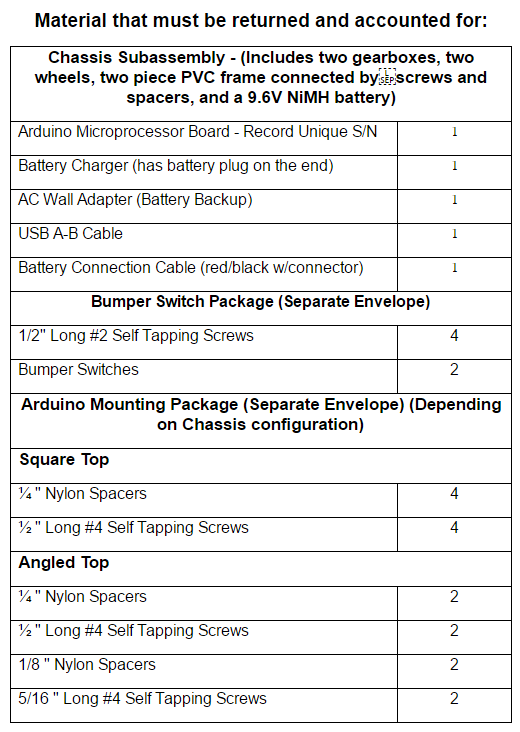
\includegraphics[height=13cm]{ReturnMaterial.png}\\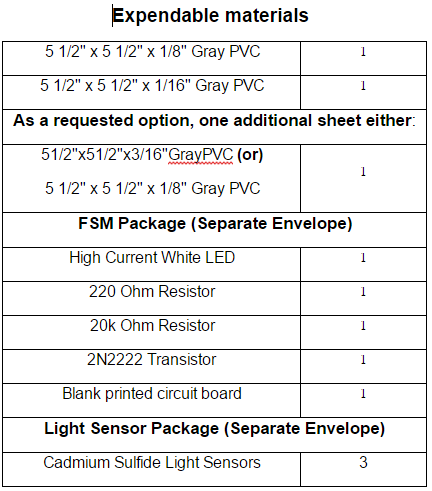
\includegraphics{ExpendableMaterials.png}}\end{center}
\subsection{System Design}
Group 1 looked at multiple designs to try and evaluate what type of overall design should be taken across the robot. Through looking at four different designs the team decided to mix up different design concepts from each section to make the strongest impact on score. While the group scored the robot designs based on conceptual criteria, looking at how fast it would cross to enemy territory or shut down lights without any testing beforehand, the results may have been skewed to our beliefs in the robot design versus technical application. \\

The group decided that programming complexity and battery drainage were not strong enough criteria to remove choices from our concepts. Therefore, while more sensors added complexity, the team decided to include three to have a stronger overall strength in extinguishing target lights. \\

The beacon light was placed at 6 inches in order to distance the readings from the light sensors and beacon sensors enough, however also keep it close to the body in order to have a more stable center of gravity and fast speed possibilities. Because two robots would be colliding with each other, the worst thing that could happen is have our robot get pushed over onto its side. \\

In order to win, the group decided that focus would be placed on making our robot as good as possible. Instead of placing countermeasures on our robot to mess with the other robots, which not only would take time from our schedule and place extra workload onto our robot, Group 1 focused on making our robot strong in its individual trials. Emphasis on strengthening our own robot was our "win strategy." The team incorporated wooden framework to strengthen its durability and create a sturdy center of mass. See below for Alternative Designs and Final Arduino I/O Wiring: \\

In our first design Group 1 looked to incorporate less target sensors and a lower beacon sensor in order to minimize the mechanical design needed for the robot as well as lower the amount of code needed to make the robot work. However, the team realized that it was not impressed with the performance it thought the robot would have. Although the robot did not draw much on the power of the robot, the issue with confusing target and beacon lights was a very big problem that this design would have to surpass.\\

The second theoretical design incorporated square bumpers and multiple target sensor lights. This design ended up being the strongest scoring, and the group used many of its design features in the full implementation of the next robot. The group did however decided to include an extra target light in order to safely navigate across the enemy territory. When looking through the positive and negatives of this design the team realized that the robot was far stronger with more sensors and therefore the group decided to focus more on adding as much data collection devices as the team needed instead of worrying about battery life or code complexity.\\

The third design  focused more on the placement of the floor sensor module and the height of the beacon sensor. The group also decided to test the implementation of a sensor in the back of the robot to make sure that it was not traveling away from sources of light. Group One learned that a floor sensor module in the back of the robot was most beneficial in the way the team was thinking about creating the robot because it wanted the full robot to cross over the enemy territory before following through with the next set of code. Also, the team decided to not include the back sensor in our final design because issues would have arose from the beacon light affecting the sensor.\\

Finally, the last design looked to incorporate more choices that the group did not look at before into the design process. For instance the team looked at the possibility of adding sensor lights only in the front and the back of the robot, however that did not bode well for the robot. Also, the pointy bumper design got caught in many turning movements and was scrapped as well. In the end the final design consisted of a mashing of multiple functioning parts to create the best, coherent design. Group One decided to make a robot with 3 sensor lights all in the front, a single beacon light nine inches from the base, a floor sensor module in the rear of the chassis and rounded bumpers with a gap in the middle. \\

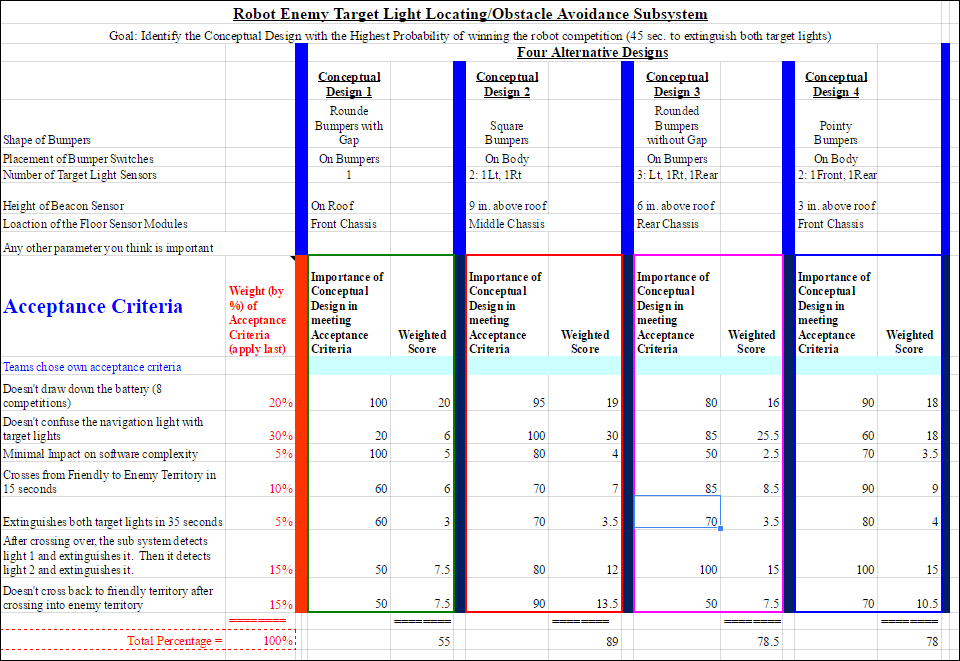
\includegraphics[width=\textwidth]{AlternativeDesigns.png}
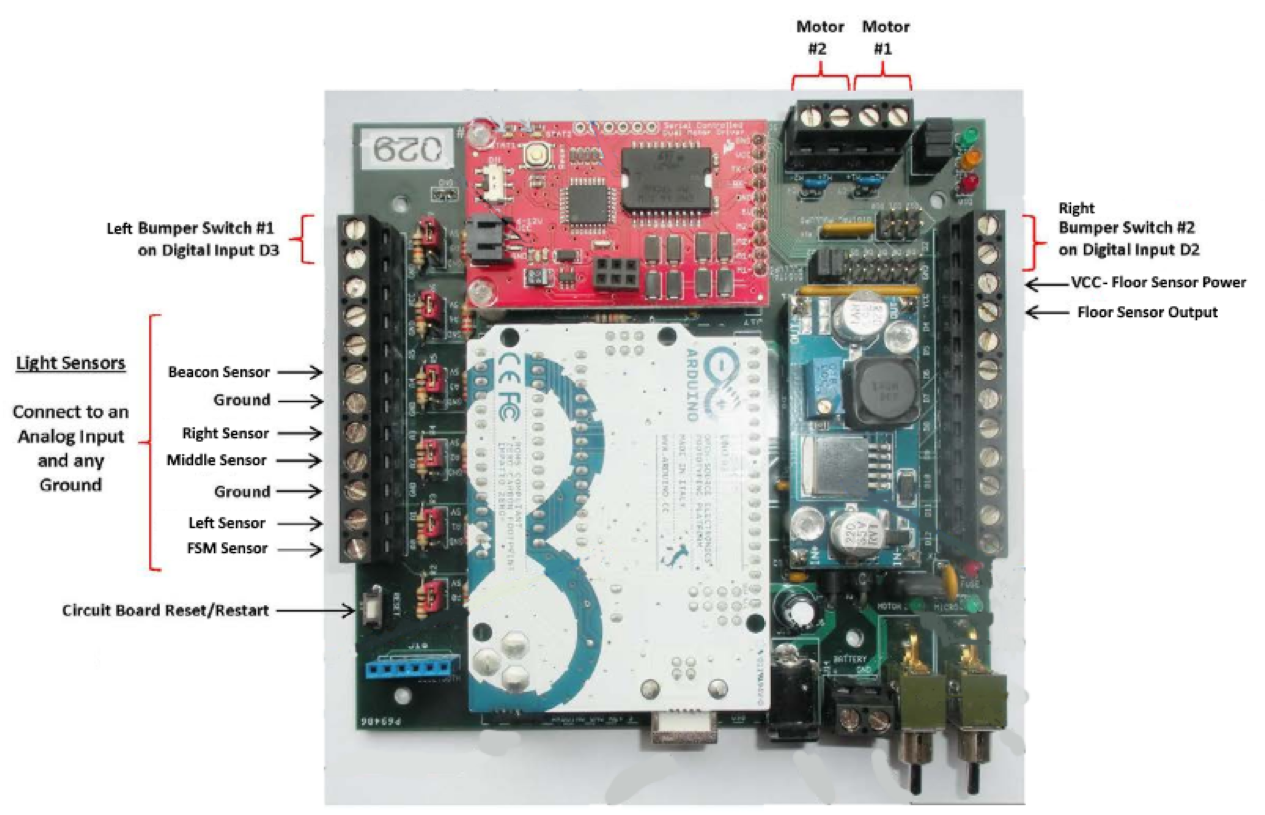
\includegraphics[width=\textwidth]{IOConnections.png}
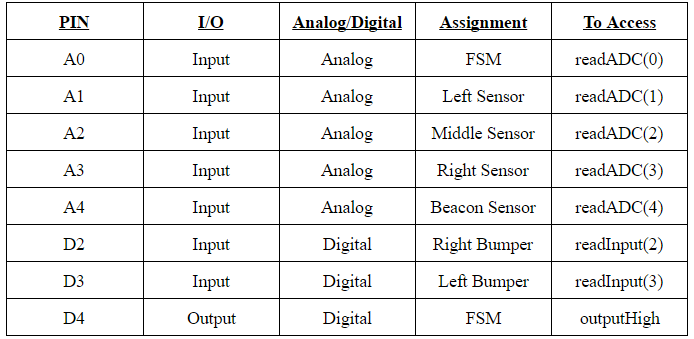
\includegraphics[width=\textwidth]{IOTable.png}
\newpage
\subsection{Mechanical Design}
The body of the robot was designed to effectively withstand the labors of the tasks necessary in competition while maintaining workmanship and aesthetic qualities. At first, the body was constructed with a white plastic cardboard material, which was somewhat flexible but very durable. When completed, however, it was sloppy looking and therefore insufficient, so it was rebuilt with wood. After this, the shields for the target light sensors were taped down with the same plastic material, yet the design was once again not aesthetically pleasing, so these were removed and replaced with wood. \\

	Other than the aforementioned changes, the design and construction of the robot went smoothly and as planned. Beginning with the bumpers, the design on Solidworks was mapped with precisely measured lines and curves, and holes were placed in the necessary positions. A two-bumper system was used, along with an under piece to hold them in place and create stability.  \\
	
	\begin{center}
	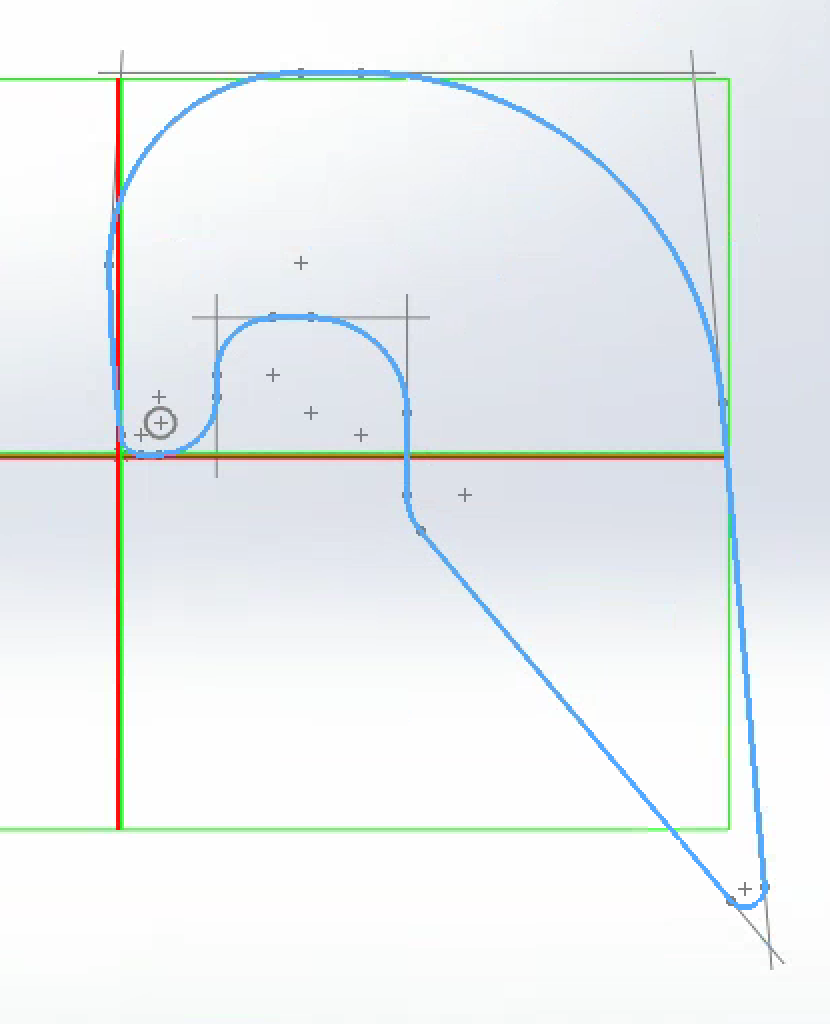
\includegraphics[height=10cm]{Bumpers.png}
	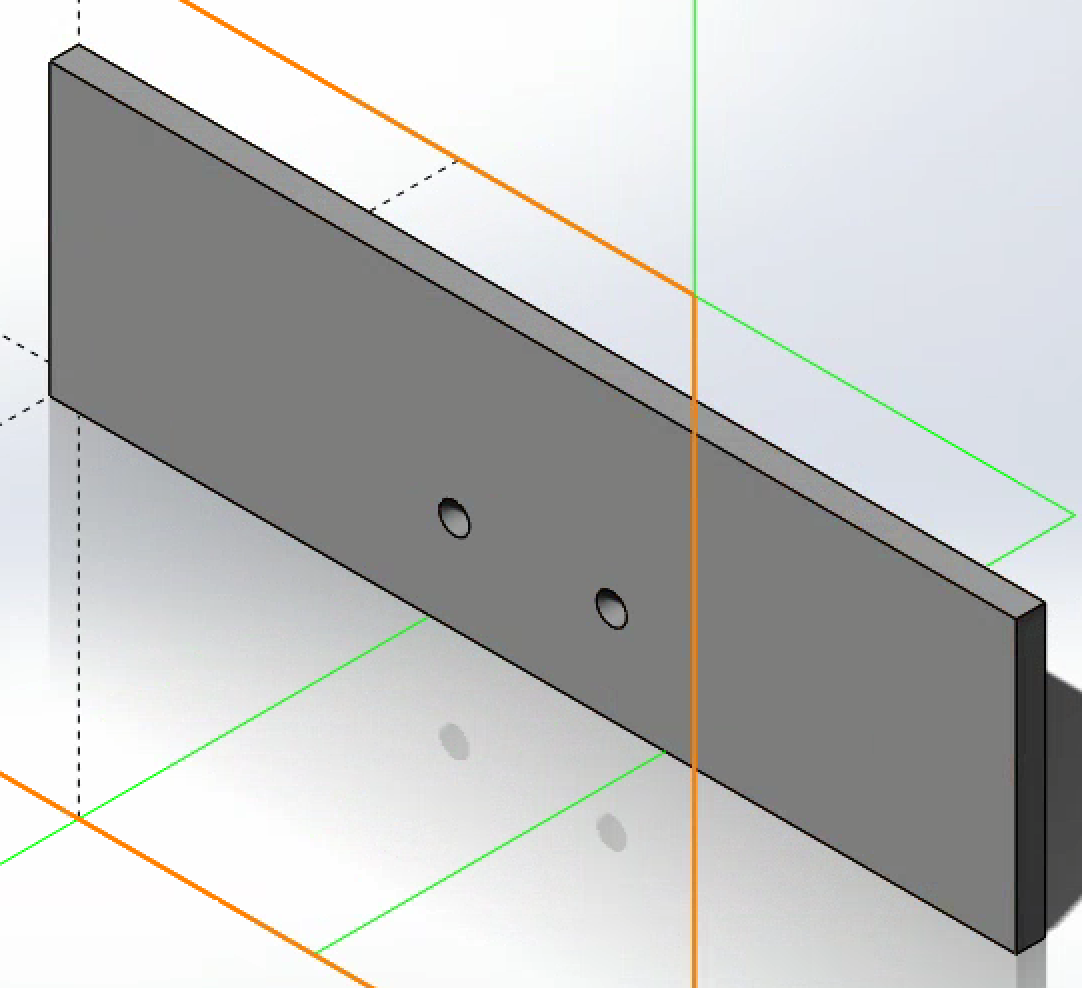
\includegraphics[height=10cm]{BumperSupport.png}
	\end{center}
	
	Next in order was the frame of the body (chassis), which was constructed using four pieces of scrap wood screwed twice each into the Arduino mainframe. The last piece of the frame was screwed four times, or once each into the four supporting beams. This piece was made of balsa wood for a sturdy body, able to support the weight of the target light sensors and the shield that’s cover them. \\
	
	The FSM was then constructed and placed on the bottom of the robot. The schematic on canvas was followed precisely and the transistor, LED, and photo resistors were all soldered into place. Then the FSM was mounted to the back-bottom of the robot using zipties. \\
	
	\begin{center}
	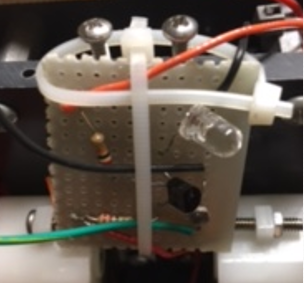
\includegraphics[width=8cm]{FSM.png}
	\end{center}
	
	Once this was completed, the shields for the target light sensors were constructed. Their shape was similar to that of a box, with an open end to be glued to the floor, and an open end to the outside that light could come through and reach the sensors. \\
	
	Finally, the tower for the beacon light sensor was cut from balsa wood. A flat piece of balsa wood nine inches in height was cut and screwed twice to the Arduino mainframe from the back, and an open box facing up was glued together attached to it in order to shield the beacon light sensor from target lights and other possible distracting lights. \\
	
	Additionally, the robot had construction done around its photo resistors to ensure shielding and less variable results. Two taller, slanted pieces of scrap wood were placed inside the open box to further obstruct the possible light sources coming in to the beacon light sensor, and to help direct the light sensor towards the beacon light. Likewise, rectangular boxes were created to surround the light sensors in the front of the robot in order to shield them from the beacon light above. One the front of the boxes was kept open to keep data incoming from the target lights.\\
	
	Finally, the logo and aesthetic parts of the robot were created both out of balsa wood, the laser cutting station, pipe cleaners, and a black sharpie. The group decided to incorporate a moustache theme around the robot and so a moustache was created in Solid Works to be etched onto a square block as our logo. Later, black sharpie and black pipe cleaner were used to create a coherent flow through the aesthetic design. A black moustache was made out of pipe cleaners and placed on top of the robot, and many of the wooden pieces build were colored in with a sharpie to make them black. \\ 
	
	\begin{center}
	
\includegraphics[height=10cm]{LOGO.png}
	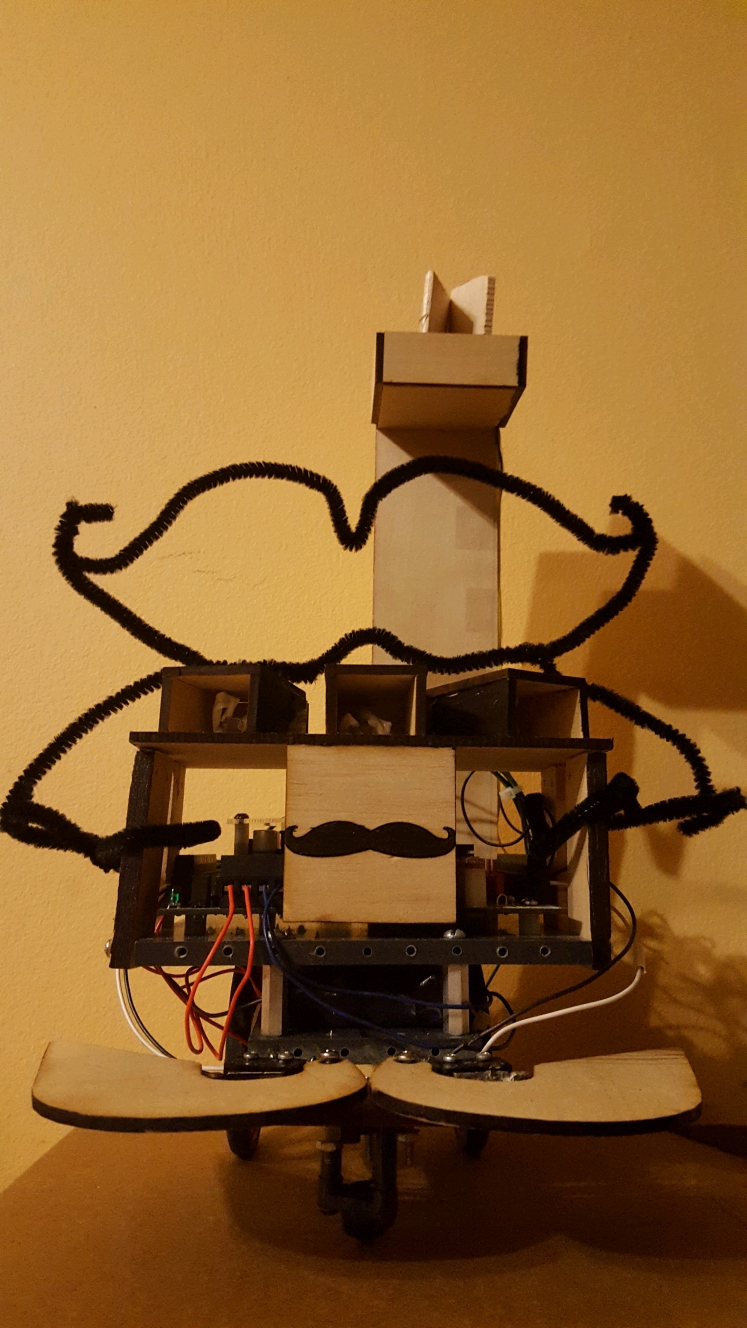
\includegraphics[height=10cm]{Robot.png}
	\end{center}
	
	Throughout this entire process, careful steps and communication were required to ensure that each participant could successfully complete his/her job with minimal difficulty due to construction. Certain areas were needed for wiring entry and soldered wires, and other areas were needed open for screwing/maintenance reasons. In whole, the mechanical design was a synthesis of each team members’ thoughts efforts. Not only was structure and durability an important factor, but constant maintenance and visually appealing design were certainly considered as well. 

\subsection{Software Design and Coding}
    After the hardware aspects of the robot were built, C programming was necessary to create functionality out of the robot. The coding process started with evaluating routines and subroutines for the robot to accomplish and then putting them together in a logical order with loops and if-statements. In order to make the coding process easier, two flowcharts were made at the start of the process to organize the procedure the robot will take and also evaluate ideas without coding to look for functionality (Made in Visio). Group 1 decided that the territory that the robot was on dictated what it should be doing and therefore most of the code revolved around first checking what territory it was on before going further into the process. 
    
    \begin{center}
    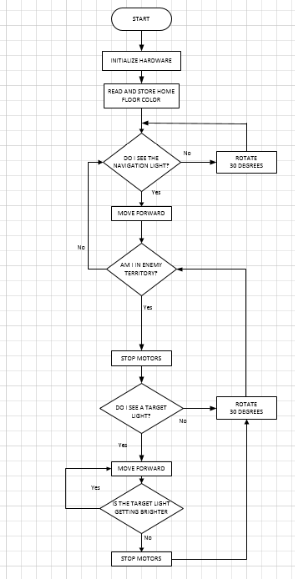
\includegraphics{MainFlowchart.png}
    \newpage
    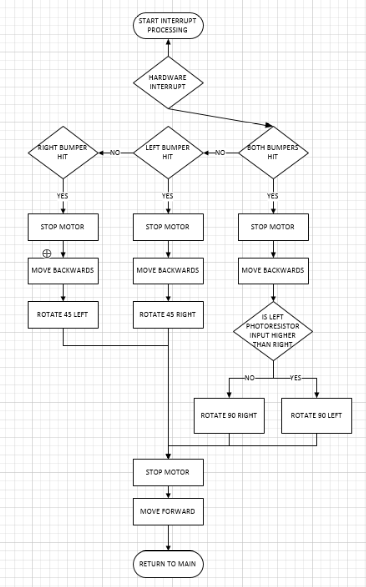
\includegraphics{BumperFlowchart.png}
    \end{center}
    

    
    Multiple routines were created in the robot based on questions the robot had to answer. These questions were also relevant when creating the flowcharts above and organizing the robots tasks. In order to make the robot fully functional, the robot had to be able to successfully solve each of these issues:\\
    
    \begin{itemize}
        \item Movement: How to Move and How to Turn?
        \item Floor Sensor Module: What Territory Am I In?
        \item Bumper Interrupt: Which Bumper was hit and where do I turn?
        \item Beacon Light: Where is the beacon light located, and how do I get there?
        \item Light Sensors: Which Way to Turn to get to the target lights?
    \end{itemize}
    
    \subsubsection{Subroutines}
    To help organize the code into a more action-based, and make it more readable, specific subroutines were made to allow the robot to do specific actions when instructed to. The subroutines ranged from simple definitions of how fast to go and how to turn left or right, to full-fledged 360 degree turns or territory checking algorithms. What made the software development unique for Group 1 was that the implementation of code was done separately from other parts of the code before being implemented into the final code. This way subroutines could be tested alone and can be singled out to look for errors. Therefore, code was not developed incrementally until finished but the code was split apart into different functions and tackled one at a time.
    
    \subsubsection{Robot Movement}
    At the beginning of the semester, an assignment was made to make the robot dance. This assignment allowed students to accompany themselves with predefined routine functions to use motors and control them to do specific operations. Below is code made specifically for the Robot Dance and an explanation of how each routine was later used in the finished robot programming.
    
    \begin{center}
    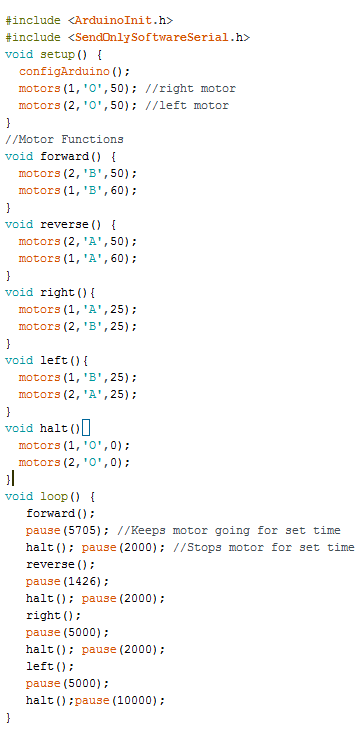
\includegraphics[]{RobotDance.png}
    \end{center}
    
    The configArduino() subroutine function allowed the robot to use pre-made custom functions \\
    
    \begin{center}
    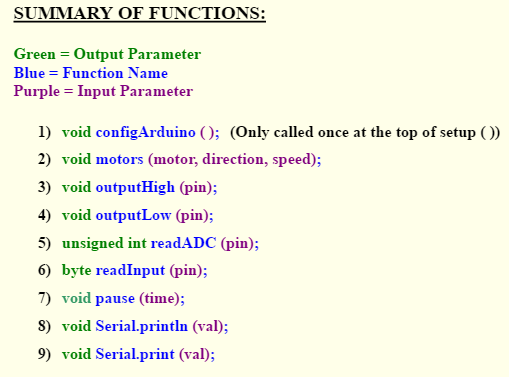
\includegraphics[]{Subroutines.png}
    \end{center}
    
    Name:  configArduino();   \\
    Purpose:  Configures the Arduino board to its baseline E121 design project configuration.  This includes setting pins 10-12 as digital outputs initialized low for the on-board LEDs, setting pins 2 & 3 as digital inputs for the bumpers, setting all remaining digital pins as inputs, all I/O ports/pins to be digital inputs, initializing the bumper interrupt function, turning off the motors and initializing then to rotate in an arbitrary direction at 100 percent full speed. Additionally the USB serial communications port to your laptop is initialized and configured for 115200 Baud.  This function MUST be called ONCE at the top of your setup ( ) function. \\
    
    Name:  motors (motor, direction, speed); \\
    Purpose:  Sets the on/off condition, direction of rotation and speed of motor #1, which physically corresponds to the terminals marked M1- and M1+, OR of motor#2, which physically corresponds to the terminals marked M2- and M2+, OR of both motors according to specified input parameter. \\
    
    outputHigh(pin); \\
Purpose:  Sets the specified I/O pin to be an output pin and initializes it to be high (logic level 1). This put 5 volts on to the output pin. \\

Name: outputLow(pin); \\
Purpose:  Sets the specified I/O pin to be an output pin and initializes it to be low (logic level 1). This connects the output pin to ground. \\

Name: unsigned int readADC(pin); \\
Purpose:  Reads the voltage present at the specified analog input pin and returns that value back to the calling function.  This function is used to read the output of the light sensors. \\

Name: byte readInput(pin); \\
Purpose:  Used to read digital inputs.  Returns the digital logic level (0 or 1) present at an input pin.  0 indicates the pin is connected to ground; 1 indicates the pin is connected to 5 VDC. \\

Name: pause(time);  \\
Purpose: To introduce a delay in the program on the order of milliseconds, 1 millisecond minimum, 65,535 milliseconds (65.535 seconds) maximum.  This function operates by timing an execution loop.  This function will not return to the calling function until the specified time interval has been reached. \\

Name: Serial.println(val); \\
Purpose:  Prints data to the USB serial port as human-readable ASCII text followed by a carriage return character (ASCII 13, or '\r') and a newline character (ASCII 10, or '\n'). This function is useful for viewing the output of your light sensors, or for general debugging purposes by viewing the value of any variable at strategic places in your program.  This function will sent data over the Arduino USB programming cable to your laptops for display on the serial monitor screen which is part of the IDE. The serial monitor must be set to 115200 baud via the pull down menu in the lower right hand corner of the monitor window. \\

Name: Serial.print(val); \\
Purpose:  Prints data to the USB serial port as human-readable ASCII text. This command operates similar to Serial.println (), but does not automatically add a carriage return/line feed to the end of your data. \\
    
    
    The pre-made function motors() helped simplify the procedures when making movement occur in the robot. For example, in the forward() function, the motors were both set to approximately half power to move the robot forward. In the reverse() function, the same occured, but the motors were flipped to rotate in the opposite direction, making the robot move backwards. By putting both the forward and reverse codes together, left and right turns could be made. Finally, a halt() function was used to stop all movement in the robot. \\
    
    After these functions were created it was much easier to code to make the robot do exactly what was needed. In order to make the robot go forward, it was much easier to call the forward() function instead of constantly including everything that was in the forward function. This also made testing and tweaking much easier as a change inside the function changed throughout all uses of the functions. In the end, the forward, halt, left, and right functions were all transfered exactly to the final robot.\\
    
    
    \subsubsection{Floor Sensor Module}
    At the start, the floor sensor module was chosen to be evaluated and coded. By installing the floor sensor module on the bottom of the robot and reading the input data on a photo resistor, a number value was collected and could be analyzed. Photo resistors increase in resistance and therefore reduce voltage when bright. These voltage numbers could then be collected by the Arduino and used in furthering the coding procedures with algorithms and actions for the robot to perform. In the case of the floor sensor module, light reading were monitored on both the light and dark areas of the field and a threshold was created that was between both of the numbers. If the number recorded by the FSM sensor was higher, it would think there was less light and assume being on the black territory, and vice versa if the FSM sensor was lower. \\
    
    \begin{center}
    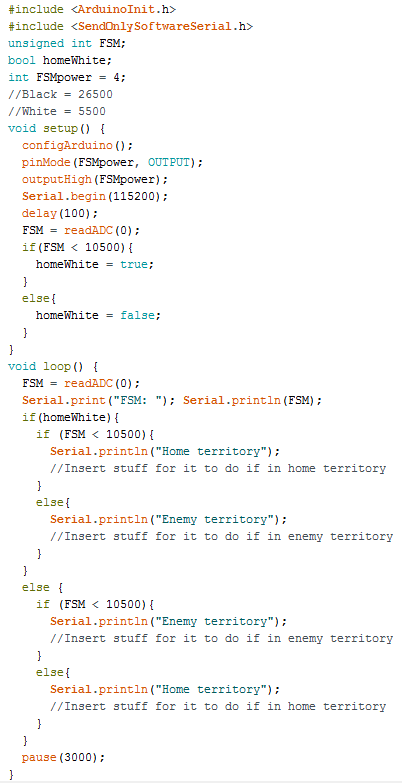
\includegraphics[]{FSMCode.png}
    \end{center}
    
    As seen by the code on the previous page, an integer variable was set to collect the photo resistor readings called FSMpower. Previous testings concluded that on the black territory FSMpower had a value of ~26500 while on white territory FSMpower had a value of ~5500. Therefore a threshold of 10500 was set that was in between both to be the deciding factor of which territory it was on. If FSMpower was below this value it was on white territory, and if above it, it was on black territory. However, that did not help it decide if it was on home territory or enemy territory. Therefore, within the setup function, which only occurs at that initiation of the robot, a value for FSM determined if the variable homeWhite = true or homeWhite = false. If the robot was placed on the white territory to start, homeWhite would be set to true and then the value of FSMpower could be used in the loop to determine home or enemy territory. Likewise, the opposite would occur if it was in the black territory for the start.
    
    \subsubsection{Bumpers}
    Next, the bumpers were taken into account. Throughout the process, the robot was expected to navigate around obstacles to reach its destination on the other side of the arena. However, because motion sensors could not be used, our robot was forced to bump into the obstacles are reach accordingly to make its way around them. The bumpers were connected to a single interrupt command which initialed whenever a bumper was hit and the switch was initiated. When the left bumper was hit, the robot was told to move backwards, and to the left simultaneously. Testing on timing with a specific speed of the motors allowed a calibration onto a rotation of 45 degrees of turning. When the robot had finished its turn, it was told to move forward for a full second before returning to its code. The same idea was implemented if the right bumper was hit, but instead the robot turned to the right. If both bumpers were hit, the robot would turn 90 degrees towards the closest light, indicated by the readings on the light sensors in front of the robot. Whichever was higher would in turn choose which way the robot turned. It is important that rotating towards the light helped not only save time, but also strengthened the readings and made the robot move more accurately towards the target lights instead of the beacon light.\\
    
     \begin{center}
    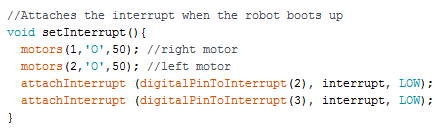
\includegraphics[]{setInterrupt.png}\\
    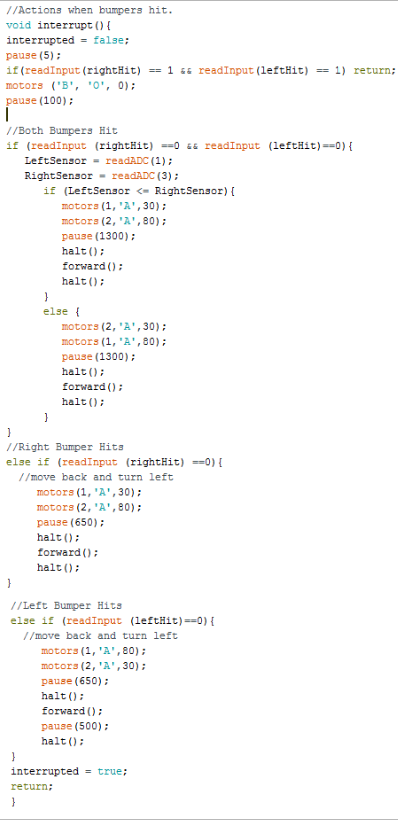
\includegraphics[]{Interrupt.png}
    \end{center}
    
    The setInterrupt() subroutine specifies what triggers the Interrupt function and attaches it to the bumper switches. This subroutine is placed within the setup() function of the code to only run at the start up of the robot. The interrupt() function, on the other hand, tells the robot what to do when it bumps into different obstacles. Furthermore, an important variable within the interrupt function is the interrupted boolean value. This value returns true if an interrupt occurred and false if it did not. Later, this is used in accordance with the beacon light to initiate a turn to check for the highest value. The next paragraph will explore this.
    
    \subsubsection{Beacon Light}
    With the bumpers completed, the robot was finally ready to incorporate light sensors into its design. First, the beacon light was used in order to make the robot cross into enemy territory. Since only one beacon light was used on our robot, it was decided that the robot should spin one full revolution at the start and gather data on the strongest light source (lowest voltage reading) onto the beacon light sensor. Then, the robot would turn again, but stop when it reached a value similar to the previously recorded light source value. A threshold of 500 was placed to ensure that it would always stop turning, however not stop too early. After the robot was centered onto the beacon light, code ensured that the robot would move forward until a bumper interrupt occurred. The idea was that the robot would constantly be going towards the light source unless an obstacle was in the way and it was forced to move away from the light source. Therefore, a boolean variable was placed within the interrupt process which returned true when an interrupt occurred and turned back into false after recalculating the strongest beacon light and centering on it. \\
    
    \begin{center}
    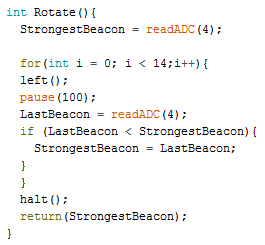
\includegraphics[]{Rotate.png} \\
    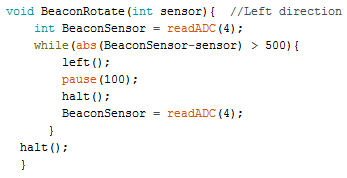
\includegraphics[]{BeaconRotate.png} \\
    \end{center}
    
    The Rotate() subroutine does the task of turning the robot in 360 degrees incrementally getting values and storing the smallest (brightest) value. This is then returned back to the BeaconRotate() function and used to turn the robot until it is at most 500 away from the highest value. This threshold was found by testing for values and found to be stable in making the robot fixate on the beacon sensor. As previously mentioned, both of these functions only happen at the setup as well as when an interrupt happens.  
    
    \subsubsection{Light Sensors}
    Finally, after the robot moved into enemy territory, the light sensors took over the movement decisions. The light sensors in the front of the robot all received values before the robot moved and let it rotate to center onto the light source. If the left sensor was higher voltage then the right sensor, which meant more light was coming from the right, the robot was told to turn right. Inside this if statement, a while statement decided how long this turn would occur for. Before each turn a "previous" sensor value was recorded and after the turn finished a "new" sensor value was recorded. If the new sensor value was brighter (smaller) than the old value, the robot would keep turning. The turning would end once the new value was not brighter than the old one. \\
    
    \begin{center}
    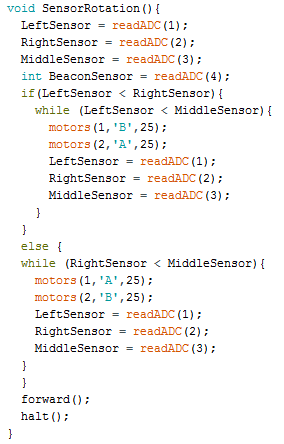
\includegraphics[]{SensorRotate.png}
    \end{center}
    
    \subsubsection{Full Code}
\begin{center}
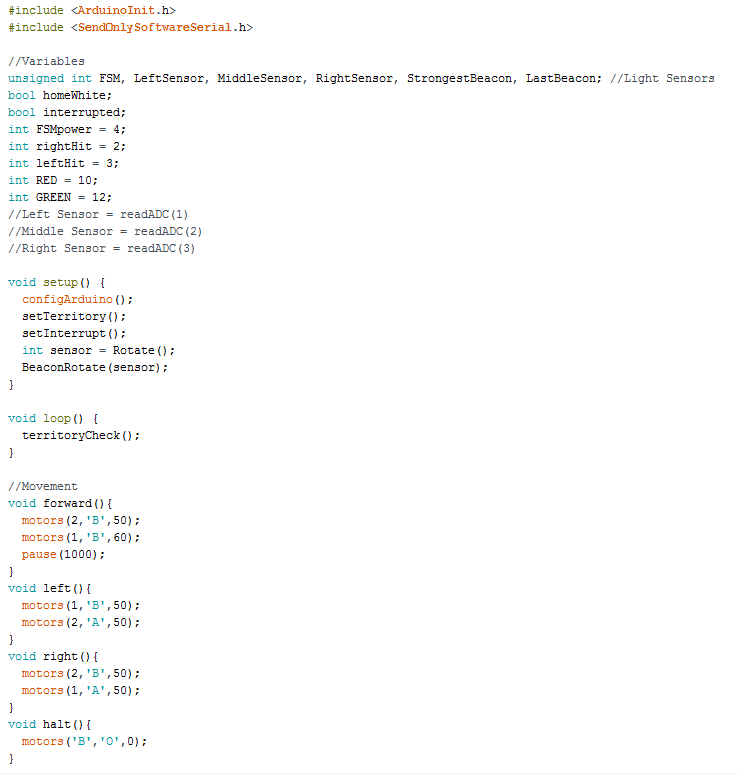
\includegraphics[width=\textwidth]{FullCode1.png}
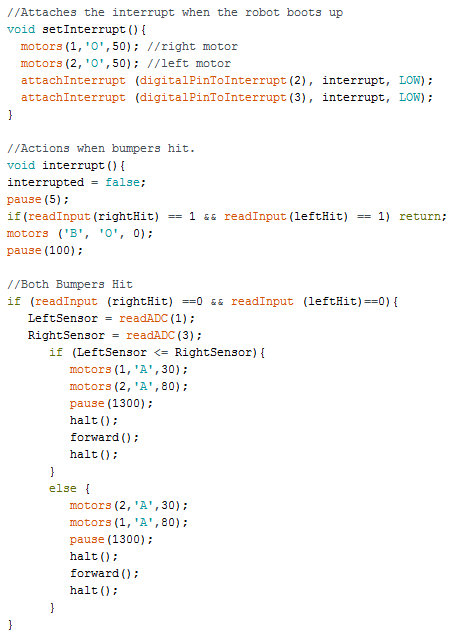
\includegraphics[]{FullCode2.png}
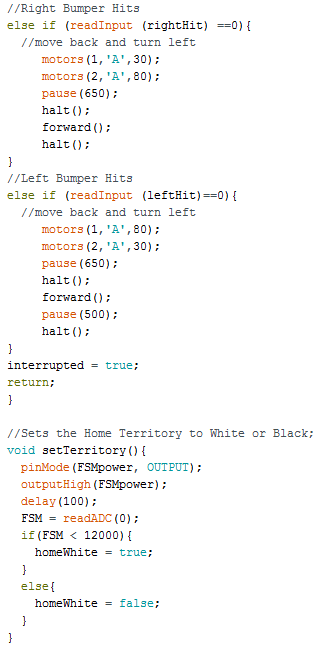
\includegraphics[]{FullCode3.png}
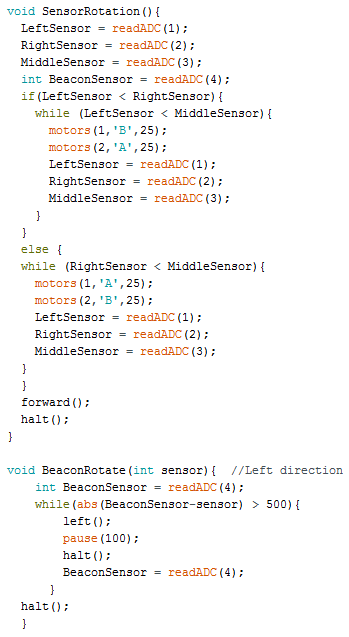
\includegraphics[]{FullCode4.png}
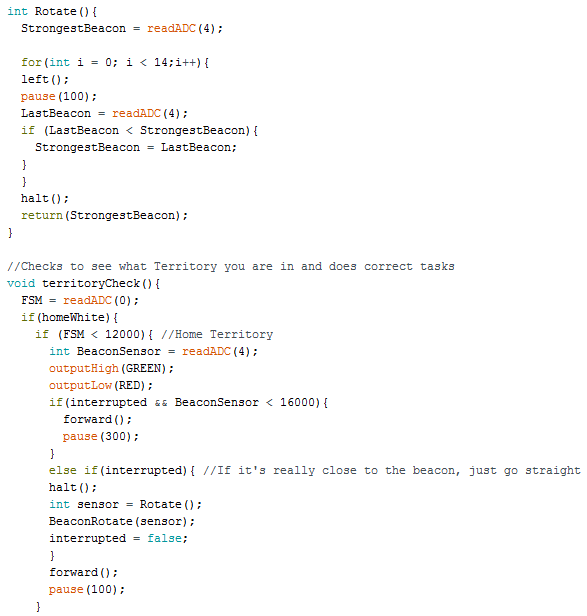
\includegraphics[]{FullCode5.png}
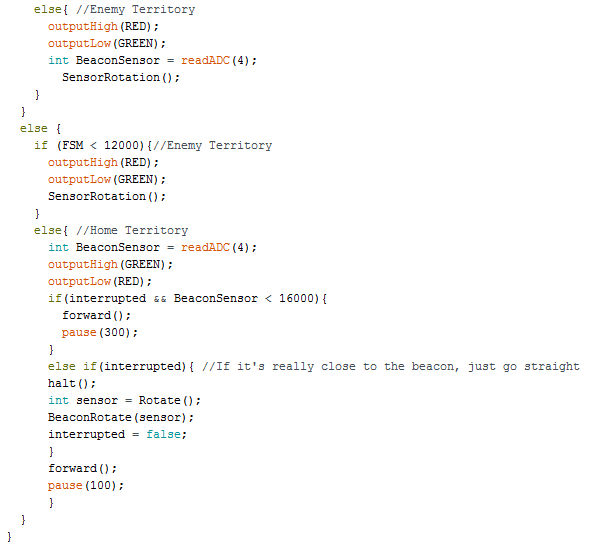
\includegraphics[]{FullCode6.png}
\end{center}
    
\subsection{Electrical and Wiring Design}
    In order to successfully implement the code and use it, many photo resistors and wiring needed to be done to the robot to make it functional on the hardware side of the project. Likewise, there needed to be a system which captured this data.
    
    \subsubsection{Arduino Board}
    Most of the electrical components that were implemented onto our robot ultimately connected with the Arduino Board. An Arduino Board is  an open-source electronics platform based on easy-to-use hardware and software. It's intended for anyone making interactive projects. What is most important however, is that Arduino senses the environment by receiving inputs from many sensors, and affects its surroundings by controlling lights, motors, and other actuators. By connecting photo resistors and motors to the Arduino Board, many of the robots functions could be interpretted and changed based on these values through the coding that has been done. To connect the arduino in order to upload code, use the given usb connector to plug into a usb slot in a computer as well as the Arduino port shown below: 
    
    \begin{center}
    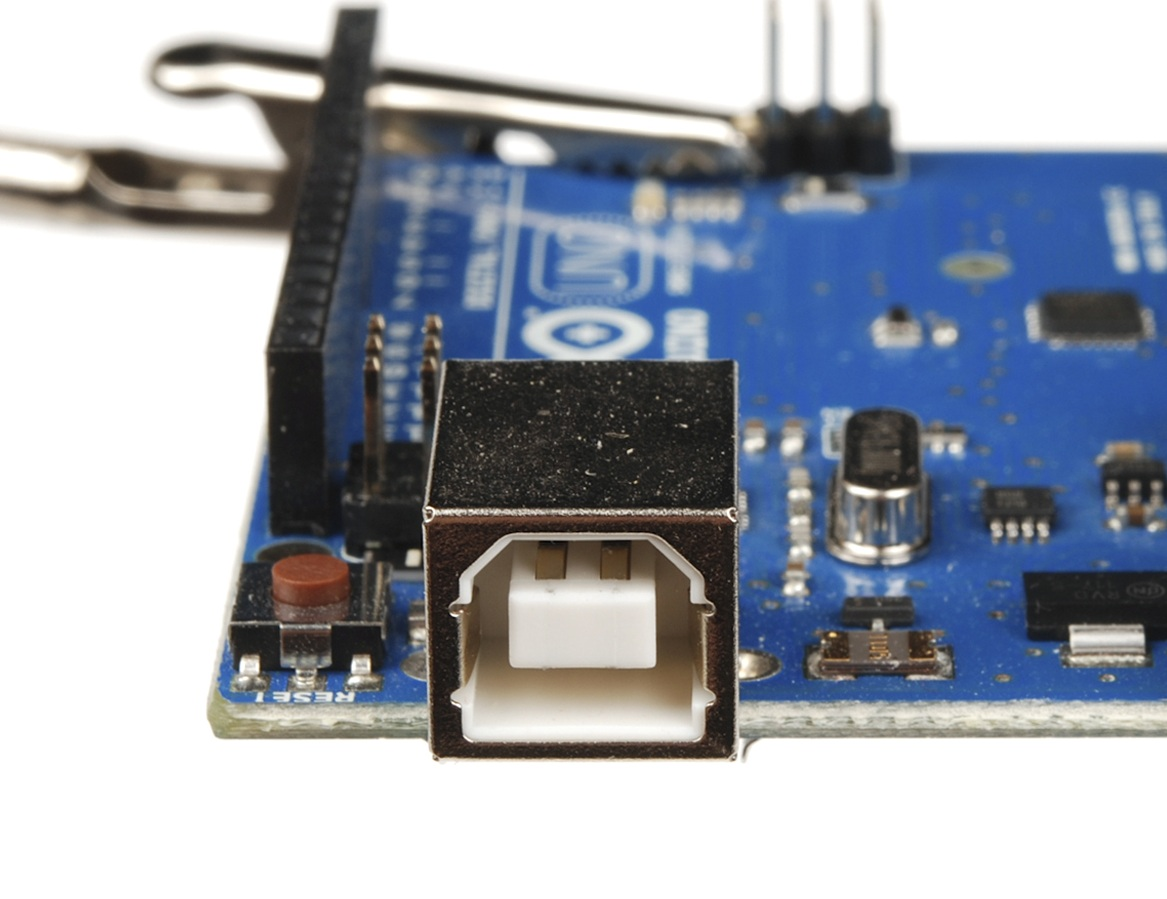
\includegraphics[]{ArdunioPort.JPG}
    \end{center}

    \subsubsection{Electrical Design}
    Four major tasks were solved by using electrical design hardware. First, photo resistors were connected in order to ensure that data could be acquired from them to use in code. Second, motors were connected in order to allow the robot to move around the arena. Third, bumper switches were connected in order to allow interrupts to be recorded when the bumper switches were hit by an obstacle. Lastly, the floor sensor module was connected with a transistor to allow for the territory to be recorded.
    
    \subsubsection{Photo Resistors}
    The light sensors supplied with the robot are cadmium sulfide devices.  A property of this material is that it acts as a “variable resistor” in the presence of light.  This means its electrical resistance, measured in ohms, is proportional to the intensity of light shining on its surface.  As the light intensity increases, the sensor’s electrical resistance decreases.  As the light intensity decreases, the sensor’s electrical resistance increases.   As electrical resistance increases, it becomes harder and harder for electrical current to pass through it.   Rubber is an example of a material that has a very high electrical resistance. In fact, it is so high that it is used as an “insulator” to protect people from the hazards of electricity. Copper on the other hand is a material that has a very low electrical resistance, which explains why it is used in wiring as a “conductor” of electricity.\\

    This variable resistance property of the light sensor is used in conjunction with a fixed resistor and a 5 volt power source located on the Arduino microprocessor board to form a simple voltage divider circuit. A typical circuit schematic of the light sensor circuitry is shown below:  (One typical circuit is depicted. The Arduino board has six of these to connect up to six light sensors.)  As the resistance of the light sensor varies, the voltage at the I/O pin will also vary.  From Ohm’s Law, voltage at the I/O pin (VI/O) can be calculated using the formula shown.  The microcontroller has internal analog to digital (A/D) converters that can measure this voltage and present the value it sees to the program.
    
    \begin{center}
    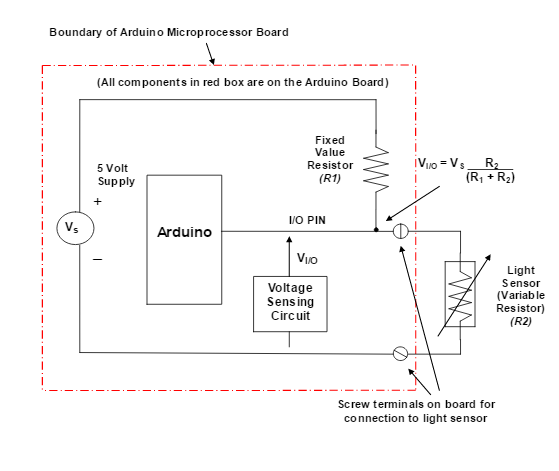
\includegraphics[]{Photoresistor.png}
    \end{center}
    
    \subsubsection{Motors and Interrupts}
    A computer interrupt is a hardware driven event.  That is, when the value (voltage) on a particular input pin of the microprocessor changes state (for example when a bumper switch closes) the internal hardware of the chip will immediately sense the event, immediately stop whatever it was doing (even counting down a delay), save the current processing environment (so it can return there later) and jump to a certain location in memory where the “interrupt service routine (ISR)” is located. The Arduino Uno has two external interrupt pins, digital inputs D2 and D3, which have been assigned to the two bumper switches.  If either pin sees a voltage change caused by a bumper switch closure, the software will immediately jump to the ISR that you design and code.  \\
    
    Your ISR logic should verify the bumper hit by reading the pin(s) and then initiate appropriate motor control actions to get around the obstacle.  Once the bumper switch(es) indicate that the obstacle has been cleared, the interrupt function will return to the main program, restore the environment that was saved when the interrupt occurred, and continue exactly where it left off.  This results in evasive action being taken immediately upon a bumper switch activation. In this case, interrupts were used to stop motors from proceeding with their regularly programmed movement and instead made them follow the procedure inside the interrupt. \\
    
    As mentioned above the Arduino Uno has two external interrupt lines that are on digital input pins D2 and D3.  The design of the microprocessor board assigns these pins to the bumper subsystem and further provides a set of screw terminals for you to easily wire in the bumper switches. (See “Interfacing to the Arduino Microprocessor”).  The switches have three connection terminals, but you will only use two of them, the ones marked C (common) and N.O. (normally open).  The third terminal N.C. (normally closed) is not used in our application. So each switch will have two wires attached to it that will be routed up and connected to the pre-assigned screw terminals. There is no polarity to a switch closure so either wire can go to either screw terminal. The wires should however be soldered to switches to ensure a good, solid connection.
    
    \subsubsection{Floor Sensor Module}
     The FSM works using a light sensor and a white high current Light Emitting Diode (LED).  Light from the LED will reflect off of the floor and hit the light sensor. The higher the intensity reflected back, the lower the light sensor reading will be. Both of these devices, as well as some supporting circuitry will be soldered to a small printed circuit board you will mount to the underside of your robot, near the arena floor. Here is the schematic for the floor sensor module: 
     
     \begin{center}
     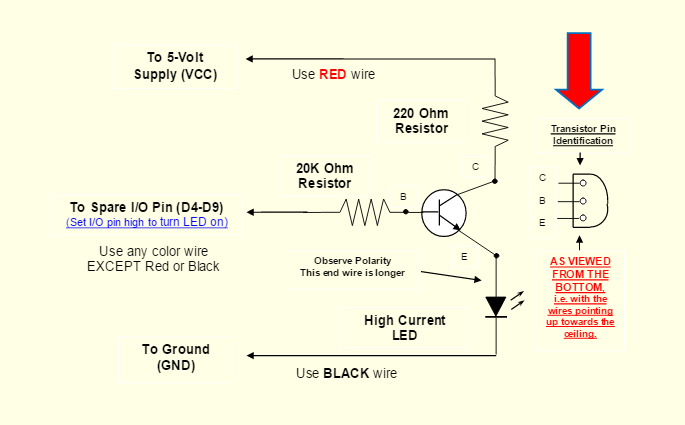
\includegraphics[width=\textwidth]{FSMSchematic.png}
     \end{center}
     
    \subsubsection{Wire Color Coding}
    While there were no unique considerations in the electrical components of the robot, Group 1 did end up color coding wires for better understanding at a glance. Red wire was used to indicate the power supply and was connected both to the battery and to digital outputs that were put onto highOutput. Black wires were used to indicate ground, or the end of a circuit. Specific ports were designed to act as ground as ports on the Arduino and so all black wires ended by going into the Arduino ground ports. Green with yellow stripes wires were used to indicate the outputs from the light sensors at the front of the robot. Data collected on its voltage was put into specific digital outputs in the robot using these wires. An orange wire was used to indicate the data output from the floor sensor module on the bottom of the robot. Finally, data received from the beacon light was sent to the digital input on the Arduino with a yellow wire. By using these colored wires, the group was quickly able to see what wires did what and made sure to not mistakenly connect the wrong ones to specific ports (for example output to ground). 

\subsection{Assembly}
    \subsubsection{Problems or Concerns}
    During the assembly of the robot many problems appeared that made the group have to re-evaluate materials, design choices, and the complexity of the design. At the very start of the assembly of the robot, a plastic cardboard was used to build the base of the robot out of. However, as the robot was designed further, this plastic cardboard was considered too aesthetically displeasing and also not structurally sound. Instead, the team opted to turn to wood to construct most of the robot's body and used both screws and wood glue to hold it together. The design choices also needed to be altered once the team got to the assembly stage, as many of the ports around the Arduino needed to stay uncovered, but a base above it still needed to be build. Finally, due to most of these assembly issues, a simpler design needed to be created to finish in time. A simple shelf-like box was created to be placed ontop of the robot and hold the light sensors, while a simple but sturdy piece of wood was used to elevate the beacon sensor. 
    
    \subsubsection{Tools Used}
    Typical tools required to complete your robot project will be provided. In addition to the lab bench tools (drill press, band/scroll saws, belt sander, etc.), a tool box with hand tools (screwdrivers, wire cutters, soldering iron/solder, etc.) was used. \\
    
    A Drill Press was used to create holes for screws in our wooden body pieces. Likewise a bandsaw was used to cut the pieces into their sizes. A laser cutting station was used for more precise measurements, including bumper construction and the creation of the logo. Finally, smaller pieces of wood were glued with wood glue onto the body of the robot to create a clean and sturdy finish.

\subsection{Integration Testing and Evaluation}
    Throughout the process of creating the robot, many features had to be tested and calibrated in order to ensure the robot worked as intended. Each of the robots electrical and software functions were tested before the competition to make sure that they worked correctly. Programming with the Serial Monitor, as well as trial testing and a block approach towards coding helped evaluate where there were issues with the robot.
    
    \subsubsection{Block Approach}
    As mentioned before, the coding aspect of the robot was split up into separate subroutines and tested independently of themselves. When testing bumpers for instance, there was no code that relied on sensors or any movement on the robot. This way, problems could be isolated and carefully examined to fix. Before moving onto future programming and electrical design, each previous step was checked to be working correctly. In other words, the beacon light was not coded until bumpers and movement were working properly and exactly as intended. \\
    
    Multiple major milestones occurred while testing code. The first milestone occurred during bumper testing, where it was decided that bumpers were completed when the interrupts correctly stopped the robot from moving forward and instead accessed their own code. Even further into the bumper testing, when each interrupt was connected successfully, the actual code for what the robot should do once it is interrupted was created and tested to work correctly. Other milestones included making sure that beacon light worked successfully and the light sensors accurately led the robot to the target lights.
    
    \subsubsection{LED troubleshooting}
    While also creating specific functions to operate the robot, LEDs were also programmed within the programs to help notify when programs were being used and when they change to new operations. For instance, one LED was programmed on the robot to change from green in home territory to red in enemy territory. If for instance, the robot showed that the enemy territory had a green LED then the troubleshooting would have proved that the code for enemy territory was never initiated and therefore should be revisited. Through the visual cues of LEDs, the robot could correctly run as intended. If not, changes could be made.
    
    \subsubsection{Calibration}
    Sensors were very difficult to work with because their values jumped inconsistently due to real life variability. Therefore, theoretical code would not always work. In order to make sure that sensors were working properly the Serial Monitor was used to read in data and real life variability could be monitored. Since values were not exactly what they were expected to be, readADC() functions displayed the values of the light sensors all around the field. Through this process, for example, Group 1 was able to notice that shielding did not fully protect the light sensors from other sources and the beacon light was far brighter than the target lights. This made the robot follow the beacon light, even after shielding and distance were placed between them, and a new idea needed to be implemented to fix it. Modifications needed to be made to how far the photo resistors were inside their shielding, and extra shielding needed to be added to the beacon sensor thanks to testing and calibration efforts. Afterwards, the robot was able to perform far more effectively in the test runs.

\subsection{Final Competition}
\subsubsection{Rules and Regulations}
The following applies to the competitions that are held intra-section, on the last day of class.  For the inter-section competition held class wide, rules and scoring will be provided at that time. \\
\begin{itemize}
    \item It is each team’s responsibility to be prepared and ready for the competition on the final day of class.  Do not expect that time will be available at the beginning of class to do any work on your robot before the competition starts.  When your instructor or T/A calls for your team to start your first competition, you will be required to compete.  Be sure to have charged batteries.
    \item Each team plays every other team in their section ONE time, a match.
    \item After the first match, you may "tweak" your robot's hardware and/or software to improve performance before your next match, so long as it does not unduly delay timely completion of the class competitions.  Tweaking implies a minor adjustment that will take no longer than 5 minutes to complete.  Your instructor or T/A shall schedule remaining matches considering which robots are ready, which are being tweaked and how much time remains during class to
complete all activities.
    \item To enter the competition, your robot must at minimum have a working and reliable collision avoidance subsystem.  This means both hardware (mechanical bumpers and electrical BIS circuit) and software (Interrupt handler) must be working.  If a robot's collision avoidance subsystem is not working properly (i.e., the robot wheels keep trying to turn while stuck up against an obstacle- a motor damaging condition), your instructor or T/A will allow approximately 10 seconds for the robot to free itself.  If it does not free itself from the obstacle within 10 seconds, the power switch on that robot will be turned off.  The competing robot will be allowed to continue on and attempt to complete its mission. The disabled robot will retain the points (if any) it has earned up until when it was powered down.  The competing robot will continue to earn points until the normal end of the match.
    \item Robots that become entangled with each other, and that prohibit free movement of each other around the arena are considered to be potentially damaging to themselves.  As in the case of a faulty collision avoidance system, your instructor or T/A will allow 10 seconds for the robots to free themselves.  If unable to, the power on both robots will be turned off and the match will end. If this is the first match between two teams and if both teams agree, a second match can be held.  If a second match is not agreed to, then the points (if any) accumulated during the first match will stand.  If a second match is agreed to, then only the points
from the second match will count. If this is the second match, the points accumulated (if any) up until when the robots were powered down will be accumulated and count. A third match will not be allowed.
    \item If a robot displays any other potentially self-damaging, non-recoverable condition (wheel falls off, robot is knocked over and no longer upright, etc.) that robot shall immediately be powered down. The competing robot will be allowed to continue on and attempt to complete its mission. The disabled robot will retain the points (if any) it has earned up until when it was powered down.  The competing robot will continue to earn points until the normal end of the match.
    \item If a robot stops during the competition for other than a potentially self-damaging event (i.e., software bug, loose power connector, dead battery, etc.) the robot shall remain untouched and disabled in the arena while the competing robot attempts to complete its mission.  Any points accumulated by the disabled robot shall count. (These types of events should have been precluded through thorough system testing.) • Once a match has commenced, no one may touch the competing robots, except in the case of potentially damaging conditions as noted above, in which case the robot will be powered down, either after 10 seconds, or immediately in the case of a non-recoverable fault.
    \item The class instructor or T/A will conduct and monitor elapsed time of each match and will award and document scoring as below. • The competition will start with a coin toss.  Winner will specify the starting location and orientation of the robot.  Loser will specify the positions of the two targets lights.  If a second match is allowed as per the rules, these responsibilities shall flip for the second match.
    \item The starting orientation of the robot must be such that the front of the robot is facing at minimum approximately 90 degrees to the right or left of a line drawn from the center of the robot to the center of the arena.  Starting robot location/orientation and position of target lights will always be symmetrical on both halves of the arena.
    \item As soon as any robot knocks out the second target light on either side of the arena, the match has ended, at which time any points earned are accumulated. • A match has a time limit of 3 minutes at which time any points earned are accumulated.
    \item If in the first match and no points are earned by either robot at the end of 3 minutes, the competing teams may opt to rerun the match, but are not required to. 
    \item If the two competing teams for whatever reason(s) both agree to stop and restart a match, or both agree to redo a completed match, they can, however only points from the second match will count.
    \item At all times the competition limit between two teams is two matches.  If no points are awarded after two matches, so be it.
    \item There can be only ONE first place winner in each section. If there is a tie, those teams must play one additional match to determine the first place winner.  If there are more than two teams tied for first place, each must play every other team tied for first place one time to accumulate points and determine the winner.    
\end{itemize}

\subsubsection{Scoring and Grading}
Scoring \\
Point accumulation is designed to reward performance.  During each match a robot will be awarded points for the following events:
\begin{itemize}
    \item Robot crosses over into enemy territory –  5 points
    \item Robot knocks out one of his opponent’s target lights – 5 points.
    \item Robot knocks out second of his opponents’ target light (wins the match) – 10 points
    \item A robot that knocks out his own home territory light(s) will be debited 2.5 points per light and the opposing team will be credited 2.5 points per light.
\end{itemize}\\

The competition grading component contributes 6 percent to your final grade.  It is a group grade.  The Canvas grade book entry for the competition allows for the range 0-10.  The grade book will internally apply the 6 percent contribution to the final grade.   The number entered in the grade book for the competition component will be determined as follows:

- After all section matches are complete, add the points accumulated by each team and then priority rank each team by the total points earned. - Apply the following :
\begin{itemize}
    \item 1st  place – 10 points to grade book (only one team)
    \item 2nd place – 8 points
    \item 3rd place – 7 points
    \item 4th place – 6 points
    \item 5th place – 5 points
    \item 6th place – 4 points
    \item All others (if any) that complete the competition – 3 point
    \item Unable to compete – 0 points
\end{itemize}

If teams tie for a position, all in that tie get the associated points and all lower teams move up in ranking.  For example if two teams tie for second place, both teams will receive the grade of 8. The next team(s) in priority rank would be in third place and receive the grade of 7.

\subsubsection{Final Robot Performance}
At the end of the semester, Group One's robot ended up doing more poorly than expected. The robot ended up the competition with 27 1/2 points and was placed in last place overall within the class. Ultimately, the robot was able to successfully finish the course on its own, however when a second robot was placed in the arena at the same time, it began to disrupt our software and hardware. For instance, during three of our runs from the eight that the team were given in the competition, the robot hit into the other robot and bumpers pushed it out of its designed course. In retrospect, the bumper design and code should have been implemented with the other robot in mind on the field. In the end our robot did not finish a run with both lights triggered off, however it did get past the other side of the arena consistently and get the first target light multiple times.

\subsubsection{Robot Design - Unsuccessful}
In the end, our robot design proved to be unsuccessful and lead our team to be in last place overall in the competition. Throughout the competition many issues occurred onto our robot from bumper malfunctions to wires getting caught in the enemy robot, to light sensors not working as expected. In our first trial against an enemy robot, the bumpers actually broke from bumping into an enemy robot and the team had to adapt to the issue that occurred. Unfortunately, the group was unable to run successfully since then. If Group One were to do the run in the future, a stronger mechanical design from the start would have solved many of the issues the group had both during its runs and during integration and testing. 

\subsubsection{Rank}
In the end, the Mustache Mobile received 8th out of 8 places in the robot competition (Last). The group learned a lot through the experience but was ultimately unsuccessful in designing a robot that could turn off all the target lights in the fastest time. 

\subsubsection{Results Matrix}
\begin{center}
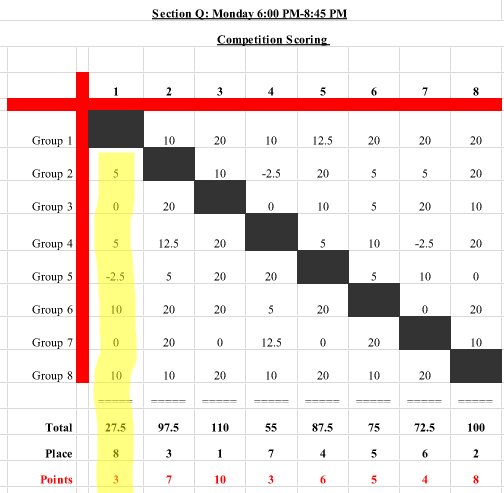
\includegraphics[width=\textwidth]{ScoringMatrix.png}
\end{center}

\section{Conclusions and Recommendations}
Throughout the competition, Group 1 learned many lessons and accomplished new ways to not only build a robot but also collaborate effectively and organize a large project together. Together, the group was successful with planning and implementing new ideas without much fighting within the group. Whenever an issue arose between group members, everyone assessed the situation and looked for the best solution. Each member was open to new ideas and also knew when they needed help or could help a struggling member. Overall, the group was able to successfully accomplish the goal of making a robot follow sensor lights and turn off the target lights. However, due to real world inconsistencies the group was unsuccessful in trying to optimize this procedure to the ideas that at first sounded correct.

\subsection{Recommendations}
Although most of the project went smoothly, a few recommendations can be made to make future projects similar to this one easier for the groups. First, our group had problems with the hardware of the robot itself, including being given small photo resistors and plastic cardboard to use for the body of the robot. In the future, larger photo resistors should be included in the bag that is given at the start of the class and a specific place should be made for materials to use to build the chassis. In the group's own experience, plastic cardboard was handed to be used for the body of the robot and was later asked to be remove because of a lack of workmanship. Previously the group believed that this plastic cardboard needed to be used.\\

Similarly, the workload split between members is skewed inconsistently between group members. For instance, in the first few classes the software member does not have much work that he can be doing. However, by the end of the project, the roles flip in intensity. Instead, a focus should be placed on making an even amount of work be organized through each class. While the mechanical engineer is working on bumpers for instance, the software member should focus on writing the code, even if the bumpers are not finished yet. \\

Finally, not enough time was put into testing the robot in the end. Multiple classes were given extra lab hours to work on their robot and fix any tweaks with it. Instead, the testing should have been started sooner, and the construction should have ended sooner as well. 

\section{Tables}
\begin{center}
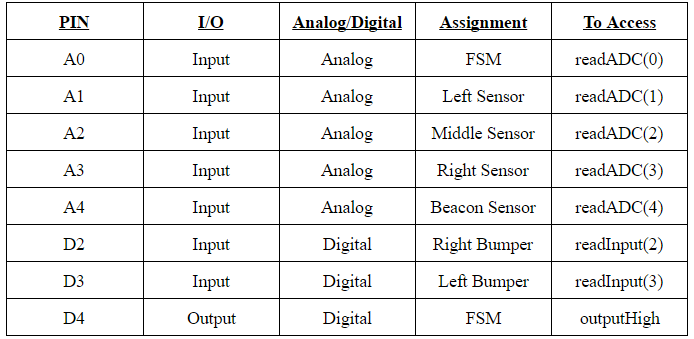
\includegraphics[width=\textwidth]{IOTable.png}
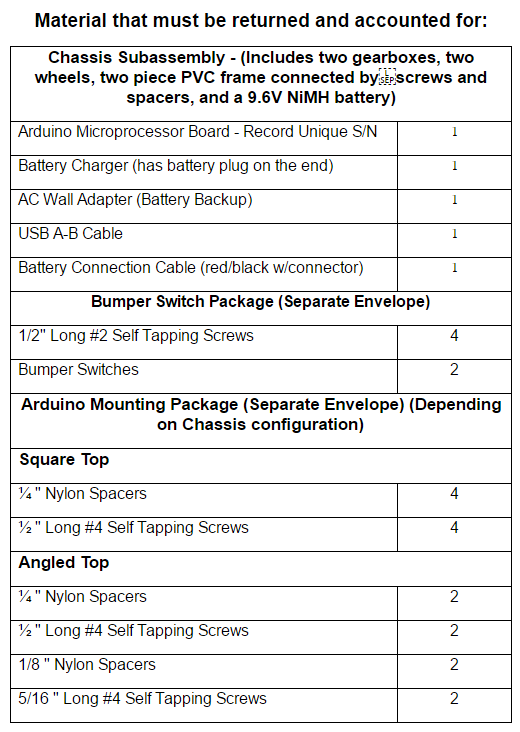
\includegraphics[height=10cm]{ReturnMaterial.png}
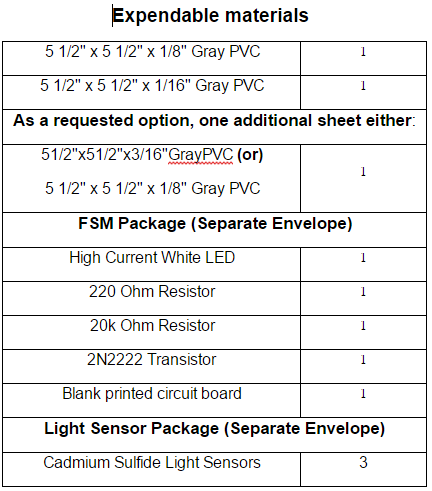
\includegraphics[height=10cm]{ExpendableMaterials.png}
\end{center}



\section{Figures}
\subsection{Arena}
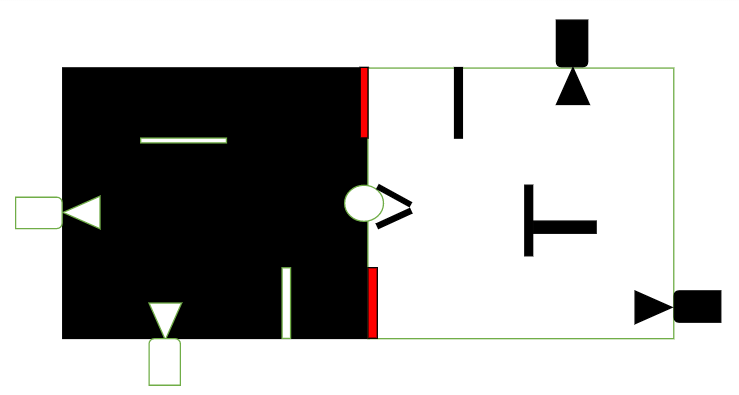
\includegraphics[width=\textwidth]{Arena.png}
\subsection{Gantt Chart}
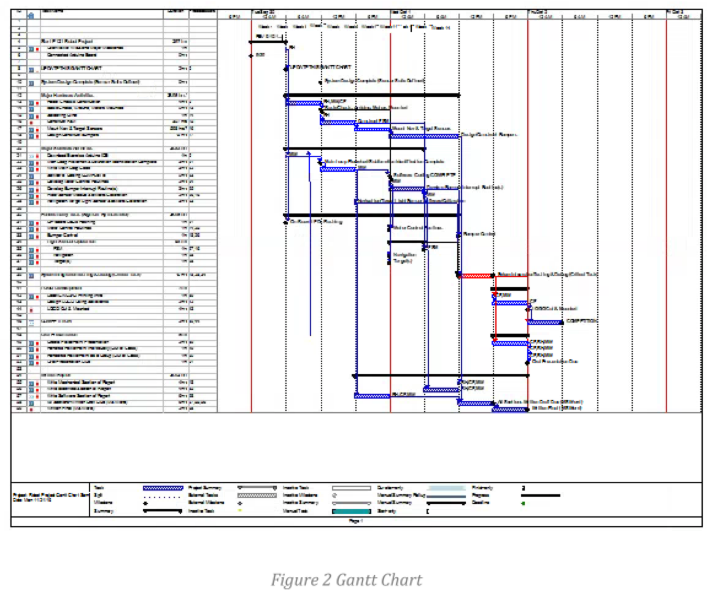
\includegraphics[width=\textwidth]{Gantt_Chart.png}
\subsection{WBS}
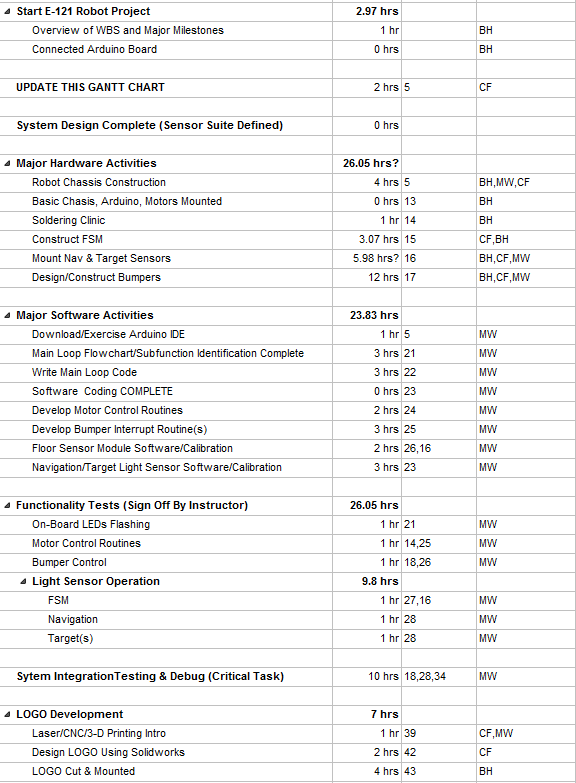
\includegraphics[height=\textheight]{GanttChartBreakdown.png}
\subsection{WBSGraphic}
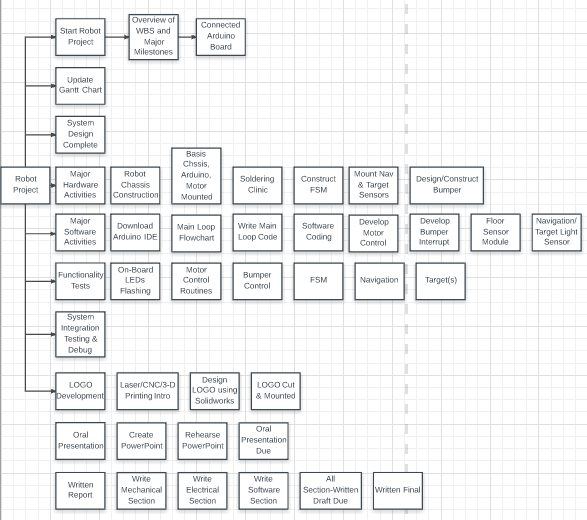
\includegraphics[width=\textwidth]{WBSGraphic.png}
\subsection{Organization Chart}
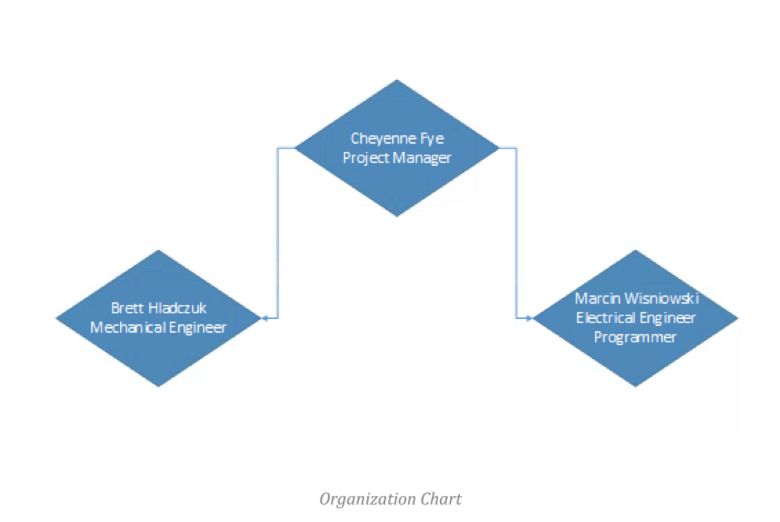
\includegraphics[width=\textwidth]{Organization_Chart.png}
\subsection{SolidWorks Bumpers}
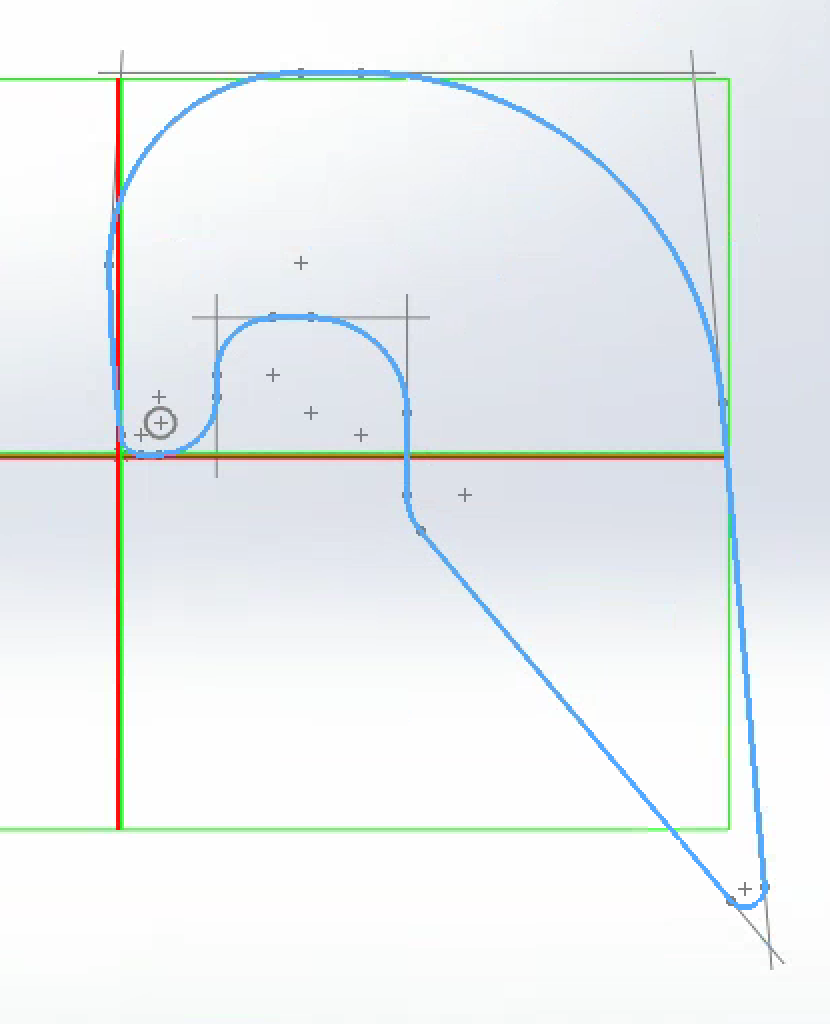
\includegraphics[width=\textwidth]{Bumpers.png}
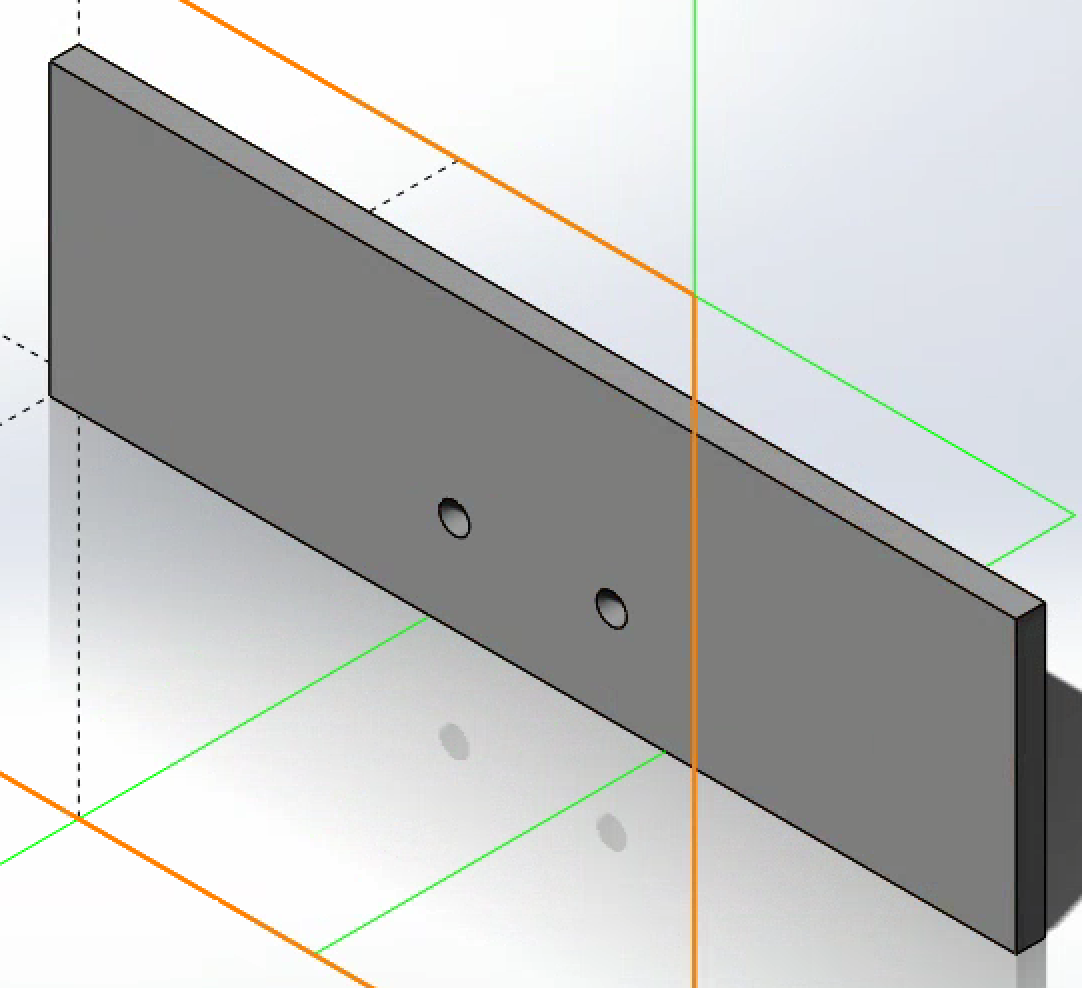
\includegraphics[width=\textwidth]{BumperSupport.png}
\subsection{Alternative Design Matrix}
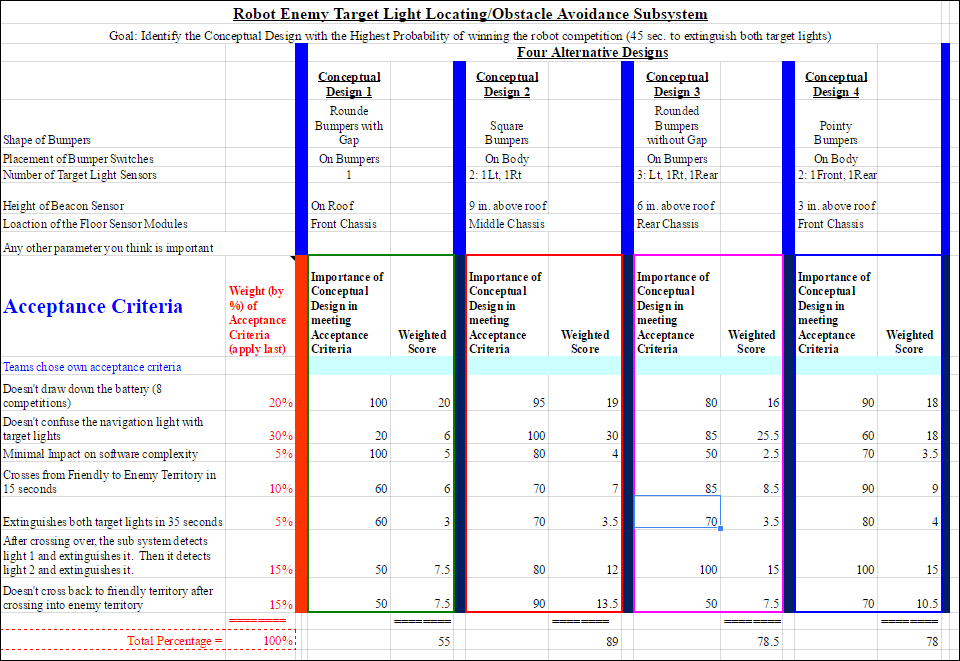
\includegraphics[width=\textwidth]{AlternativeDesigns.png}
\subsection{Body}
\begin{center}
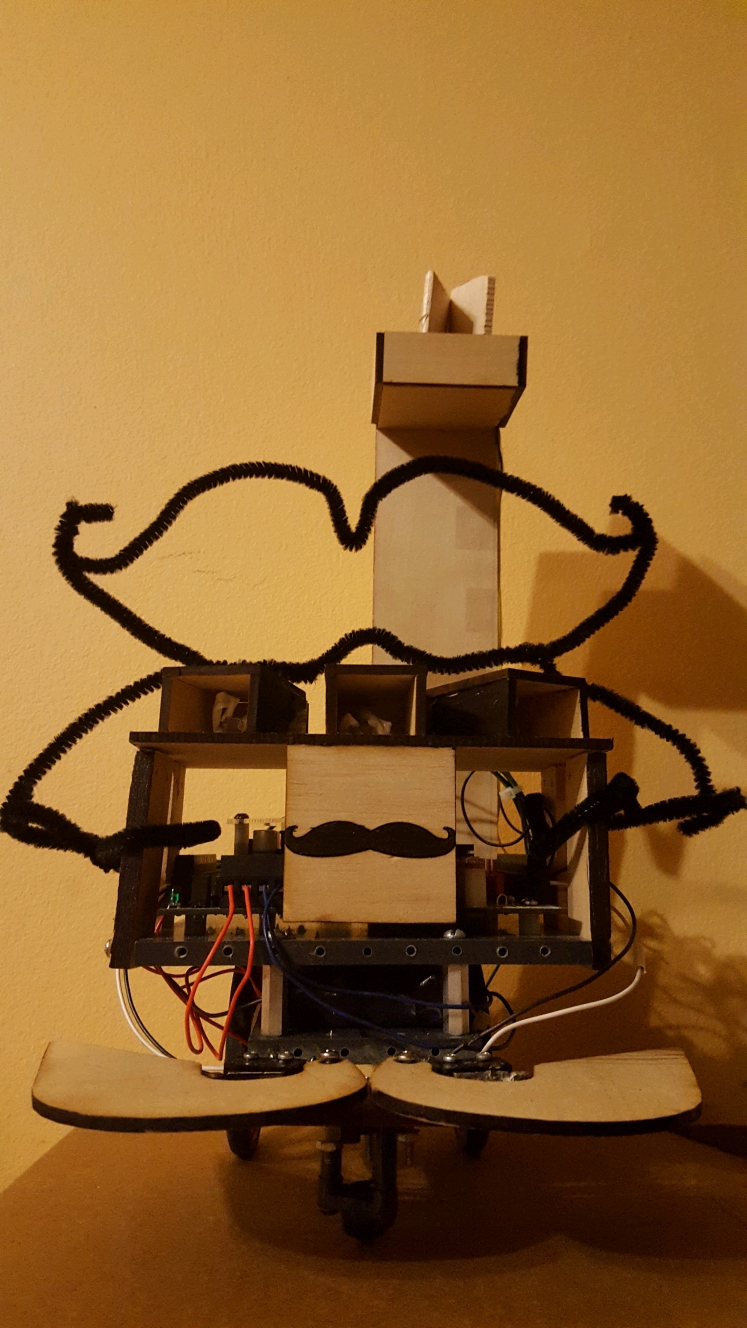
\includegraphics[height=\textheight]{Robot.png}
\end{center}
\subsection{LOGO Design}

\includegraphics[width=\textwidth]{LOGO.png}
\subsection{Bumper Flowchart}
\begin{center}
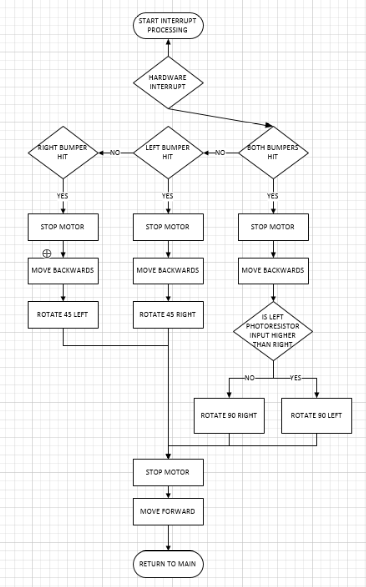
\includegraphics[height=20cm]{BumperFlowchart.png}
\end{center}
\subsection{Main Loop Flowchart}
\begin{center}
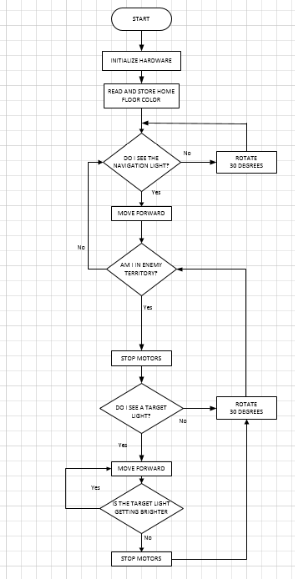
\includegraphics[height=\textheight]{MainFlowchart.png}
\end{center}
\subsection{Arduino Connections}
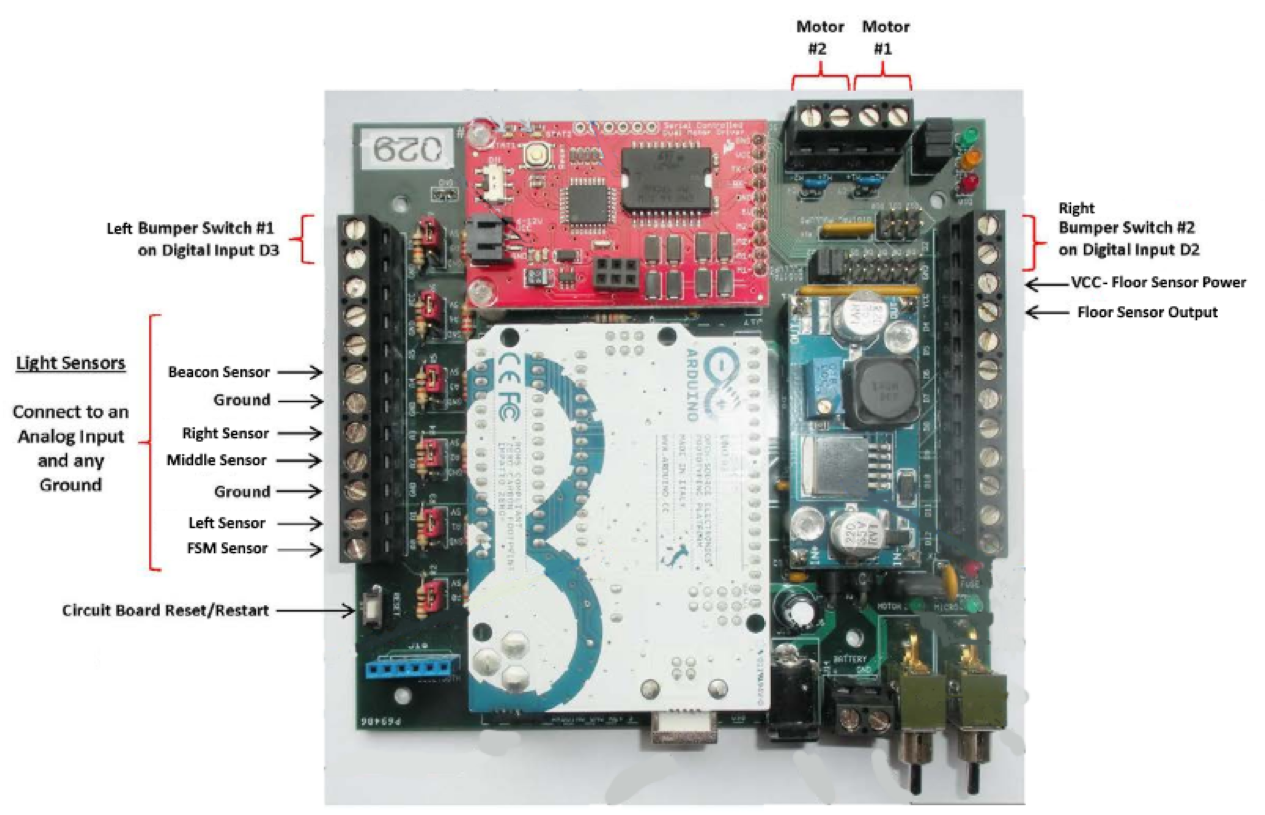
\includegraphics[width=\textwidth]{IOConnections.png}
\subsection{FSM Circuit}
\includegraphics[width=\textwidth]{FSMSchematic.png}
\subsection{Voltage Divider Circuit}
\includegraphics[width=\textwidth]{Photoresistor.png}

\newpage
\setcounter{page}{1}
\renewcommand{\thepage}{A-\arabic{page}}
\section{Attachments}
\subsection{Gantt Chart}
\includegraphics[width=\textwidth]{Gantt_Chart.png}
\subsection{WBS}
\includegraphics[height=\textheight]{GanttChartBreakdown.png}
\subsection{Organization Chart}
\includegraphics[width=\textwidth]{Organization_Chart.png}
\subsection{Bumper Flowchart}
\begin{center}
\includegraphics[height=20cm]{BumperFlowchart.png}
\end{center}
\subsection{Main Loop Flowchart}
\begin{center}
\includegraphics[height=\textheight]{MainFlowchart.png}
\end{center}
\subsection{LOGO Design}
\includegraphics[width=\textwidth]{LOGO.png}
\subsection{Full Code}
\begin{center}
\includegraphics[width=\textwidth]{FullCode1.png}
\includegraphics[]{FullCode2.png}
\includegraphics[]{FullCode3.png}
\includegraphics[]{FullCode4.png}
\includegraphics[]{FullCode5.png}
\includegraphics[]{FullCode6.png}
\end{center}



\end{document}
